\chapter{Sprint 2 : Gestion des demandes}
\section{Introduction}
Après avoir établi les fondations d'accès et d'administration dans le Sprint 1, le Sprint 2 se concentre sur la gestion des demandes au sein de la plateforme. Ce chapitre détaille les fonctionnalités prévues pour permettre aux utilisateurs, managers et RH de gérer efficacement les demandes et congés, tout en offrant des outils pour la consultation et le traitement de ces demandes. Nous aborderons les besoins, la conception et les étapes de réalisation de ce sprint.
\section{Backlog du Sprint 2}
\begin{table}[!ht]
\begin{adjustwidth}{-2.5cm}{-2.5cm}
\centering
\caption{Backlog du Sprint 2}
\label{tab:backlog_sprint2}
\begin{tabular}{ | m{5cm} | m{1cm} | m{5.5cm} | }
\hline
\cellcolor[rgb]{0.832,0.832,0.832}Cas d'utilisation & \cellcolor[rgb]{0.832,0.832,0.832}Priorité & \cellcolor[rgb]{0.832,0.832,0.832}Tâche \\
\hline
Gérer son profil & 2 & Modifier ses informations (nom, prénom, e-mail, etc.) \\
\hline
Réinitialiser son mot de passe & 2 & Utilisateur réinitialise via un lien sécurisé \\
\hline
Soumettre une demande & 2 & Utilisateurs, Managers, RH soumettent des demandes \\
\hline
Consulter ses demandes & 2 & Utilisateurs, Managers, RH consultent l’historique \\
\hline
Consulter ses congés & 2 & Utilisateurs, Managers, RH consultent congés, solde \\
\hline
Traiter une demande & 2 & Managers, RH valident ou rejettent les demandes \\
\hline
\end{tabular}
\end{adjustwidth}
\end{table}
\section{Rafinnement de cas d'utilisation }
Cette partie consiste à analyser et spécifier les besoins de ce deuxième sprint à travers l’identification des acteurs et le raffinement des cas d’utilisations.
\subsection{Identification des acteurs du deuxième sprint}
Les acteurs de ce sprint sont : \\
\textbf{Utilisateur} : Soumet des demandes (congés, absences) et consulte ses propres demandes et congés. \\
\textbf{Manager} : Soumet, consulte et traite les demandes (validation/rejet). \\
\textbf{RH (Ressources Humaines)} : Soumet, consulte et traite les demandes, gère les congés.
\subsection{Raffinement du Cas d'Utilisation <<Gérer son Profil>>}
La figure~\ref{fig:usecaseGP} illustre le diagramme de cas d'utilisation « Gérer le profil ».
\begin{figure}[h]
     \centering
     \fbox{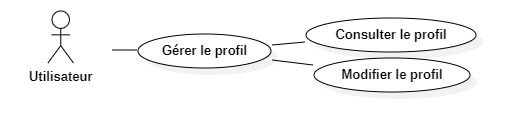
\includegraphics[width=11cm]{images/UMPRFL.jpg}}
     \caption{Diagramme du cas d'utilisation <<Gérer le profil>>}
     \label{fig:usecaseGP}
\end{figure}\\
\begin{table}[!ht]
\centering
\caption{Description textuelle du Cas d’utilisation «Consulter le Profil»}
\label{tab:view_profile}
\renewcommand{\arraystretch}{1.2}
\begin{tabular}{|p{4.2cm}|p{11cm}|}
\hline
\textbf{Cas d'utilisation} & Consulter le Profil \\
\hline
\textbf{Acteur} & Utilisateur, Manager, RH\\
\hline
\textbf{Pré-conditions} & Système en marche. \newline Utilisateur authentifié. \\
\hline
\textbf{Post-conditions} & Profil consulté. \\
\hline
\textbf{Scénario de Base} & 
1. Le système affiche l'interface du profil de l'utilisateur. \newline
2. L'utilisateur consulte la liste des informations de son profil. \\
\hline
\textbf{Exceptions} & 
Échec de consultation (problème dans l’API GET, problème dans la base de données). \\
\hline
\end{tabular}
\end{table}
Le tableau~\ref{tab:view_profile} illustre la description textuelle du cas d’utilisation « Consulter le Profil ».
\newpage
Le tableau~\ref{tab:edit_profile} illustre la description textuelle du cas d’utilisation « Modifier le Profil ».
\begin{table}[!ht]
\centering
\caption{Description textuelle du Cas d’utilisation «Modifier le Profil»}
\label{tab:edit_profile}
\renewcommand{\arraystretch}{1.2}
\begin{tabular}{|p{4.2cm}|p{11cm}|}
\hline
\textbf{Cas d'utilisation} & Modifier le Profil \\
\hline
\textbf{Acteur} & Utilisateur \\
\hline
\textbf{Pré-conditions} & Système en marche. \newline Utilisateur authentifié. \\
\hline
\textbf{Post-conditions} & Profil modifié. \\
\hline
\textbf{Scénario de Base} & 
1. Le système affiche l'interface du profil de l'utilisateur. \newline
2. L'utilisateur modifie les informations choisies. \newline
3. L'utilisateur clique sur le bouton « Modifier ». \newline
4. Le système modifie ces informations. \newline
5. Le système affiche un message de succès de modification. \\
\hline
\textbf{Exceptions} & 
Échec de modification (problème dans l’API PUT, problème dans la base de données). \\
\hline
\end{tabular}
\end{table}
\subsection{Raffinement du Cas d'Utilisation <<Réinitialiser son Mot de Passe>>}
La figure~\ref{fig:usecase_reset_password} illustre le diagramme de cas d'utilisation « Réinitialiser son Mot de Passe ».
\begin{figure}[h]
     \centering
     \fbox{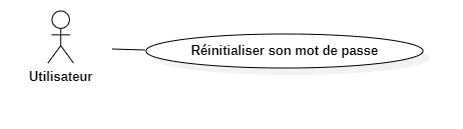
\includegraphics[width=11cm]{images/resetP.jpg}}
     \caption{Diagramme du cas d'utilisation <<Réinitialiser son Mot de Passe>>}
     \label{fig:usecase_reset_password}
\end{figure}\\
Le tableau~\ref{tab:reset_password} illustre la description textuelle du cas d’utilisation « Réinitialiser son Mot de Passe ».
\newpage
\begin{table}[!ht]
\centering
\caption{Description textuelle du Cas d’utilisation «Réinitialiser son Mot de Passe»}
\label{tab:reset_password}
\renewcommand{\arraystretch}{1.2}
\begin{tabular}{|p{4.2cm}|p{11cm}|}
\hline
\textbf{Cas d'utilisation} & Réinitialiser son Mot de Passe \\
\hline
\textbf{Acteur} & Utilisateur \\
\hline
\textbf{Pré-conditions} & Système en marche. \newline Utilisateur inscrit avec un e-mail valide. \\
\hline
\textbf{Post-conditions} & Mot de passe réinitialisé. \\
\hline
\textbf{Scénario de Base} & 
1. L’utilisateur clique sur « Mot de passe oublié » sur la page de connexion. \newline
2. Il entre son adresse e-mail et soumet la demande. \newline
3. Le système envoie un lien sécurisé à l’e-mail de l’utilisateur. \newline
4. L’utilisateur clique sur le lien et entre un nouveau mot de passe. \newline
5. Le système enregistre le nouveau mot de passe et affiche un message de succès. \\
\hline
\textbf{Exceptions} & 
Échec de réinitialisation (e-mail invalide, lien expiré, problème API). \\
\hline
\end{tabular}
\end{table}

\subsection{Raffinement du Cas d'Utilisation <<Soumettre une Demande>>}
La figure~\ref{fig:usecase_submit_request} illustre le diagramme de cas d'utilisation « Soumettre une Demande ».
\begin{figure}[h]
     \centering
     \fbox{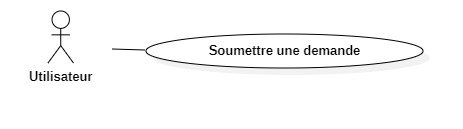
\includegraphics[width=11cm]{images/SMD.jpg}}
     \caption{Diagramme du cas d'utilisation <<Soumettre une Demande>>}
     \label{fig:usecase_submit_request}
\end{figure}\\
Le tableau~\ref{tab:submit_request} illustre la description textuelle du cas d’utilisation « Soumettre une Demande ».
\newpage
\begin{table}[!ht]
\centering
\caption{Description textuelle du Cas d’utilisation «Soumettre une Demande»}
\label{tab:submit_request}
\renewcommand{\arraystretch}{1.2}
\begin{tabular}{|p{4.2cm}|p{11cm}|}
\hline
\textbf{Cas d'utilisation} & Soumettre une Demande \\
\hline
\textbf{Acteur} & Utilisateur, Manager, RH \\
\hline
\textbf{Pré-conditions} & Système en marche. \newline Acteur authentifié. \\
\hline
\textbf{Post-conditions} & Demande enregistrée et parties concernées notifiées. \\
\hline
\textbf{Scénario de Base} & 
1. L’acteur accède au formulaire de soumission. \newline
2. L’acteur sélectionne le type de demande : \newline
   \quad a. \textit{Demande de Congé} : Formulaire avec les champs (dates de début et fin, type de congé, motif). \newline
   \quad b. \textit{Demande d’Autorisation} : Formulaire avec les champs (date, durée). \newline
3. Il remplit les détails selon le formulaire correspondant. \newline
4. Il soumet la demande. \newline
5. Le système enregistre la demande et notifie les parties concernées. \\
\hline
\textbf{Exceptions} & 
Échec de soumission (données invalides, erreur API). \\
\hline
\end{tabular}
\end{table}
\subsection{Raffinement du Cas d'Utilisation <<Consulter ses Demandes>>}
La figure~\ref{fig:usecase_view_requests} illustre le diagramme de cas d'utilisation « Consulter ses Demandes ».
\begin{figure}[h]
     \centering
     \fbox{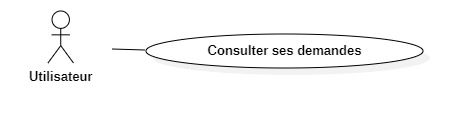
\includegraphics[width=11cm]{images/CSD.jpg}}
     \caption{Diagramme du cas d'utilisation <<Consulter ses Demandes>>}
     \label{fig:usecase_view_requests}
\end{figure}\\
Le tableau~\ref{tab:view_requests} illustre la description textuelle du cas d’utilisation « Consulter ses Demandes ».
\newpage
\begin{table}[!ht]
\centering
\caption{Description textuelle du Cas d’utilisation «Consulter ses Demandes»}
\label{tab:view_requests}
\renewcommand{\arraystretch}{1.2}
\begin{tabular}{|p{4.2cm}|p{11cm}|}
\hline
\textbf{Cas d'utilisation} & Consulter ses Demandes \\
\hline
\textbf{Acteur} & Utilisateur, Manager, RH \\
\hline
\textbf{Pré-conditions} & Système en marche. \newline Acteur authentifié. \\
\hline
\textbf{Post-conditions} & Historique des demandes affiché. \\
\hline
\textbf{Scénario de Base} & 
1. L’acteur accède à la section « Mes Demandes ». \newline
2. Le système affiche la liste des demandes avec leur statut. \\
\hline
\textbf{Exceptions} & 
Échec de consultation (erreur API). \\
\hline
\end{tabular}
\end{table}
\subsection{Raffinement du Cas d'Utilisation <<Consulter ses Congés>>}
La figure~\ref{fig:usecase_view_leaves} illustre le diagramme de cas d'utilisation « Consulter ses Congés ».
\begin{figure}[h]
     \centering
     \fbox{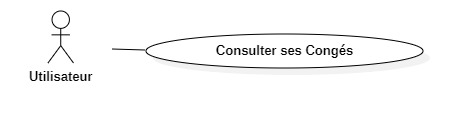
\includegraphics[width=11cm]{images/CSC.jpg}}
     \caption{Diagramme du cas d'utilisation <<Consulter ses Congés>>}
     \label{fig:usecase_view_leaves}
\end{figure}\\
Le tableau~\ref{tab:view_leaves} illustre la description textuelle du cas d’utilisation « Consulter ses Congés ».
\begin{table}[!ht]
\centering
\caption{Description textuelle du Cas d’utilisation «Consulter ses Congés»}
\label{tab:view_leaves}
\renewcommand{\arraystretch}{1.2}
\begin{tabular}{|p{4.2cm}|p{11cm}|}
\hline
\textbf{Cas d'utilisation} & Consulter ses Congés \\
\hline
\textbf{Acteur} & Utilisateur, Manager, RH \\
\hline
\textbf{Pré-conditions} & Système en marche. \newline Acteur authentifié. \\
\hline
\textbf{Post-conditions} & Solde et historique des congés affichés. \\
\hline
\textbf{Scénario de Base} & 
1. L’acteur accède à la section « Mes Congés ». \newline
2. Le système affiche le solde et l’historique des congés. \\
\hline
\textbf{Exceptions} & 
Échec de consultation (erreur API). \\
\hline
\end{tabular}
\end{table}
\newpage
\subsection{Raffinement du Cas d'Utilisation <<Traiter une Demande>>}
La figure~\ref{fig:usecase_process_request} illustre le diagramme de cas d'utilisation « Traiter une Demande ».
\begin{figure}[h]
     \centering
     \fbox{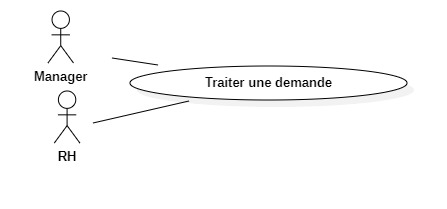
\includegraphics[width=11cm]{images/process_request.jpg}}
     \caption{Diagramme du cas d'utilisation <<Traiter une Demande>>}
     \label{fig:usecase_process_request}
\end{figure}\\
Le tableau~\ref{tab:process_request} illustre la description textuelle du cas d’utilisation « Traiter une Demande ».
\begin{table}[!ht]
\centering
\caption{Description textuelle du Cas d’utilisation «Traiter une Demande»}
\label{tab:process_request}
\renewcommand{\arraystretch}{1.2}
\begin{tabular}{|p{4.2cm}|p{11cm}|}
\hline
\textbf{Cas d'utilisation} & Traiter une Demande \\
\hline
\textbf{Acteur} & Manager, RH \\
\hline
\textbf{Pré-conditions} & Système en marche. \newline Acteur authentifié. \\
\hline
\textbf{Post-conditions} & Statut de la demande mis à jour et émetteur notifié. \\
\hline
\textbf{Scénario de Base} & 
1. L’acteur accède à la liste des demandes en attente. \newline
2. Il sélectionne une demande. \newline
3. Il choisit de valider ou rejeter. \newline
4. Le système met à jour le statut et notifie l’émetteur. \\
\hline
\textbf{Exceptions} & 
Échec de traitement (erreur API). \\
\hline
\end{tabular}
\end{table}
\section{Conception}
La conception du Sprint 2 vise à modéliser les interactions entre les demandes, les congés et les notifications, en s’appuyant sur une architecture orientée objet et une intégration avec Camunda pour la gestion des processus.\\
\subsection{Diagramme de classe du sprint 2}
La figure~\ref{fig:class_diagram_sprint2} illustre le diagramme de classe du Sprint 2.\\
\newpage
\begin{figure}[h]
     \centering
     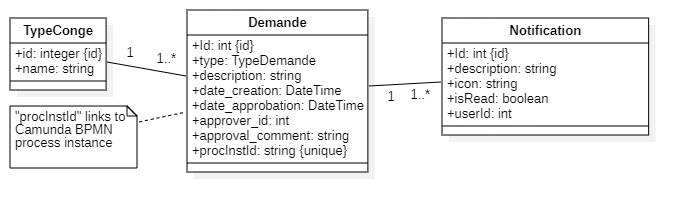
\includegraphics[width=15cm]{images/s2.jpg}
     \caption{Diagramme de classe du Sprint 2}
     \label{fig:class_diagram_sprint2}
\end{figure}
Le diagramme de classe est formé de :
\begin{itemize}
    \item \textbf{Classe "TypeConge"} : Représente les différents types de congés disponibles sur la plateforme.
    \item \textbf{Classe "Demande"} : Gère les demandes soumises par les utilisateurs, comme les congés ou autorisations.
    \item \textbf{Classe "Notification"} : Gère les notifications envoyées aux utilisateurs pour les informer sur leurs demandes.
    \item \textbf{Note sur \texttt{procInstId}} : L’attribut \texttt{procInstId} est un identifiant unique qui lie une instance de la classe (e.g., \texttt{TypeConge} et \texttt{Demande}) à une instance de processus BPMN dans Camunda. Cela permet de suivre et de gérer le workflow associé (e.g., approbation de demande) via le moteur Camunda.
\end{itemize}
\subsection{Conception du Cas d'Utilisation «Gérer son Profil»}
La figure~\ref{fig:class_manage_profile} illustre le diagramme de classe du cas d’utilisation « Gérer son Profil ».

\subsubsection{Diagramme de Classe}
\begin{figure}[h]
     \centering
     \fbox{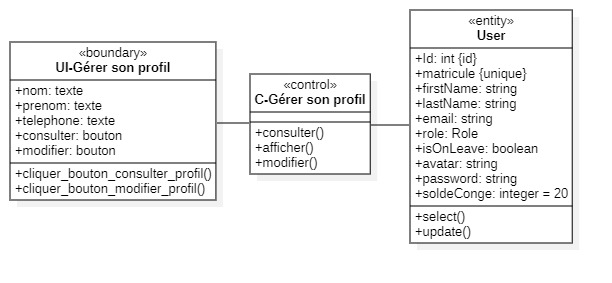
\includegraphics[width=10cm]{images/C_gerer profil.jpg}}
     \caption{Diagramme de classe du cas d'utilisation <<Gérer son Profil>>}
     \label{fig:class_manage_profile}
\end{figure}

\subsubsection{Diagramme de Séquence}
Tous les acteurs (Utilisateur, Manager, RH) ont la possibilité de gérer leurs profils à partir de leurs interfaces respectives. Lorsqu’un acteur consulte ou modifie son profil, l’interface communique avec le contrôleur de profil, qui interagit avec l’entité « User » pour récupérer ou mettre à jour les informations dans la base de données.\\
Ce scénario est présenté dans la figure~\ref{fig:seq_manage_profile}, intitulé « diagramme de séquence du cas d’utilisation Gérer son Profil ».
\begin{figure}[h]
     \centering
     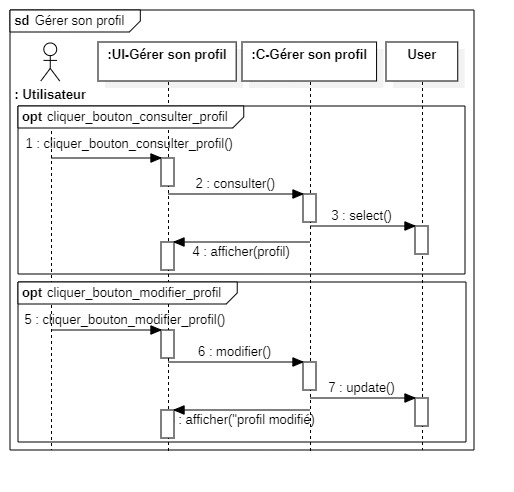
\includegraphics[width=13cm]{images/S_Gerer son profil.jpg}
     \caption{Diagramme de séquence du cas d'utilisation <<Gérer son Profil>>}
     \label{fig:seq_manage_profile}
\end{figure}
\newpage
\subsection{Conception du Cas d'utilisation «Réinitialiser son mot de passe»}
\subsubsection{Diagramme de Classe}
La figure~\ref{fig:class_reset_password} illustre le diagramme de classe du cas d’utilisation « Réinitialiser son mot de passe ».
\begin{figure}[h]
     \centering
     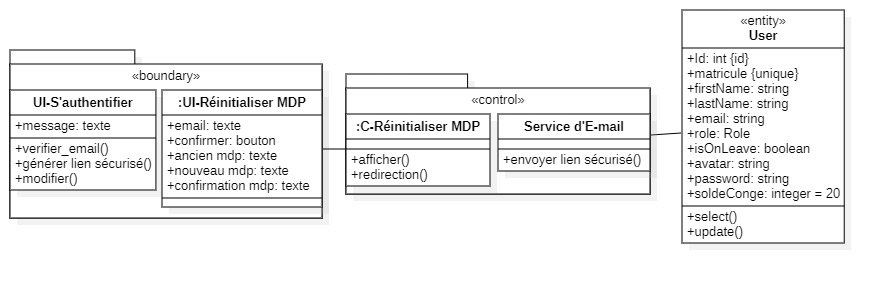
\includegraphics[width=17cm]{images/c_reset.jpg}
     \caption{Diagramme de classe du cas d'utilisation <<Réinitialiser son Mot de Passe>>}
     \label{fig:class_reset_password}
\end{figure}
\subsubsection{Diagramme de Séquence}
L’utilisateur qui a oublié son mot de passe initie le processus via l’interface de connexion. L’interface communique avec le contrôleur, qui vérifie l’e-mail de l’utilisateur dans l’entité « User ». Si l’e-mail n’existe pas, le système renvoie un message : « Si votre e-mail existe dans la base, vous recevrez un e-mail pour réinitialiser votre mot de passe », afin de ne pas divulguer l’existence de l’e-mail pour des raisons de sécurité. Si l’e-mail existe, le contrôleur génère un lien sécurisé et envoie une notification par e-mail via un service. Un attaquant potentiel recevant le lien sans connaître le propriétaire de l’e-mail ne peut pas modifier le mot de passe, car l’utilisateur doit resaisir son adresse e-mail pour confirmer son identité. Une fois le lien utilisé, l’utilisateur soumet un nouveau mot de passe, qui est mis à jour dans la base de données via le contrôleur. Après cette mise à jour, le lien devient expiré pour des raisons de sécurité. Ce scénario est présenté dans la figure~\ref{fig:seq_reset_password}, intitulé diagramme de séquence du cas d’utilisation « Réinitialiser son Mot de Passe ».
\begin{figure}[ht]
     \centering
     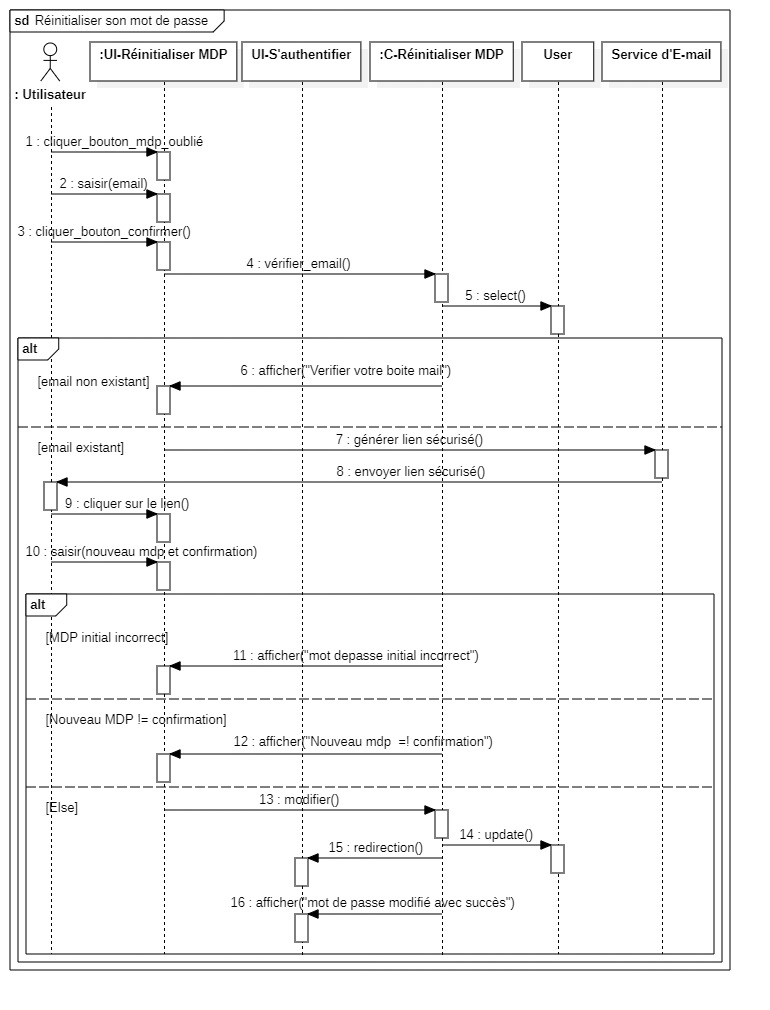
\includegraphics[width=17cm, height=0.9\textheight, keepaspectratio]{images/s_reset.jpg}
     \caption{Diagramme de séquence du cas d'utilisation <<Réinitialiser son Mot de Passe>>}
     \label{fig:seq_reset_password}
\end{figure}
\clearpage
\subsection{Conception du Cas d'Utilisation «Soumettre une Demande»}
\subsubsection{Diagramme de Classe}
La figure~\ref{fig:class_submit_request} illustre le diagramme de classes du cas d'utilisation « Soumettre une demande ».
\begin{figure}[h]
     \centering
     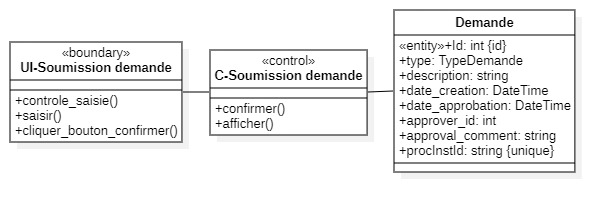
\includegraphics[width=17cm]{images/C-Soumission demande.jpg}
     \caption{Diagramme de classe du cas d'utilisation <<Soumettre une demande>>}
     \label{fig:class_submit_request}
\end{figure}
\subsubsection{Diagramme de Séquence}
Ce scénario décrit le processus de soumission d’une demande de congé par un utilisateur via l’interface de l’application. L’utilisateur commence par remplir un formulaire de demande (étape 1). La saisie est ensuite contrôlée (étape 2) pour vérifier la validité des données. En cas d’erreur, un message est affiché (étape 3) et l’utilisateur peut corriger sa saisie, dans une boucle de validation.

Une fois les données correctement saisies (étape 4), l’utilisateur clique sur le bouton de confirmation (étape 5). Cette action est capturée par le contrôleur de soumission (C-Soumission demande), qui déclenche la méthode confirmer() (étape 6). Le contrôleur interagit ensuite avec le module de gestion des demandes (Demande) pour insérer la nouvelle demande dans la base de données via insert() (étape 7).

Parallèlement, un processus BPMN est initié dans Camunda BPM afin d’orchestrer la suite du workflow de validation (par exemple, affectation de la demande à un manager pour approbation). Enfin, un message de confirmation est retourné à l’interface pour informer l’utilisateur que sa demande a été créée avec succès (étape 8).\\
La figure~\ref{fig:sequence_submit_request}, intitulé diagramme de séquence du cas d’utilisation « Soumettre une Demande ».
\newpage
\begin{figure}[ht]
     \centering
     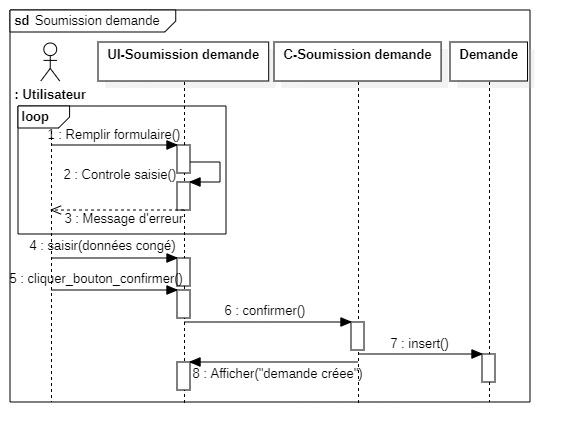
\includegraphics[width=17cm, height=0.9\textheight, keepaspectratio]{images/S_Soumission demande.jpg}
     \caption{Diagramme de séquence du cas d'utilisation <<Soumettre une demande>>}
     \label{fig:sequence_submit_request}
\end{figure}
\subsubsection{Diagramme Business Process Model and Notation}
Le diagramme BPMN ci-dessous illustre le processus métier de gestion des demandes et annulations de congé dans la plateforme. Il est structuré en deux grands processus : Demande de congé et Annulation de congé, chacun réparti entre plusieurs rôles (ou swimlanes), notamment le Manager, le service RH, et l’initiateur de l’annulation.
\paragraph{Demande de congé :}
Le processus débute par la soumission d’une demande par l’utilisateur. Celle-ci est d'abord examinée par le Manager, qui peut soit approuver, soit rejeter la demande.

En cas de rejet, le processus s’arrête immédiatement.

En cas d’approbation, la demande est transmise au RH pour une seconde validation. Si le RH rejette la demande, le processus s’arrête également.

En cas de double approbation (Manager + RH), une tâche de type service est exécutée pour mettre à jour les données du congé dans le système, marquant la fin du processus.
\newpage
\begin{figure}[h]
     \centering
     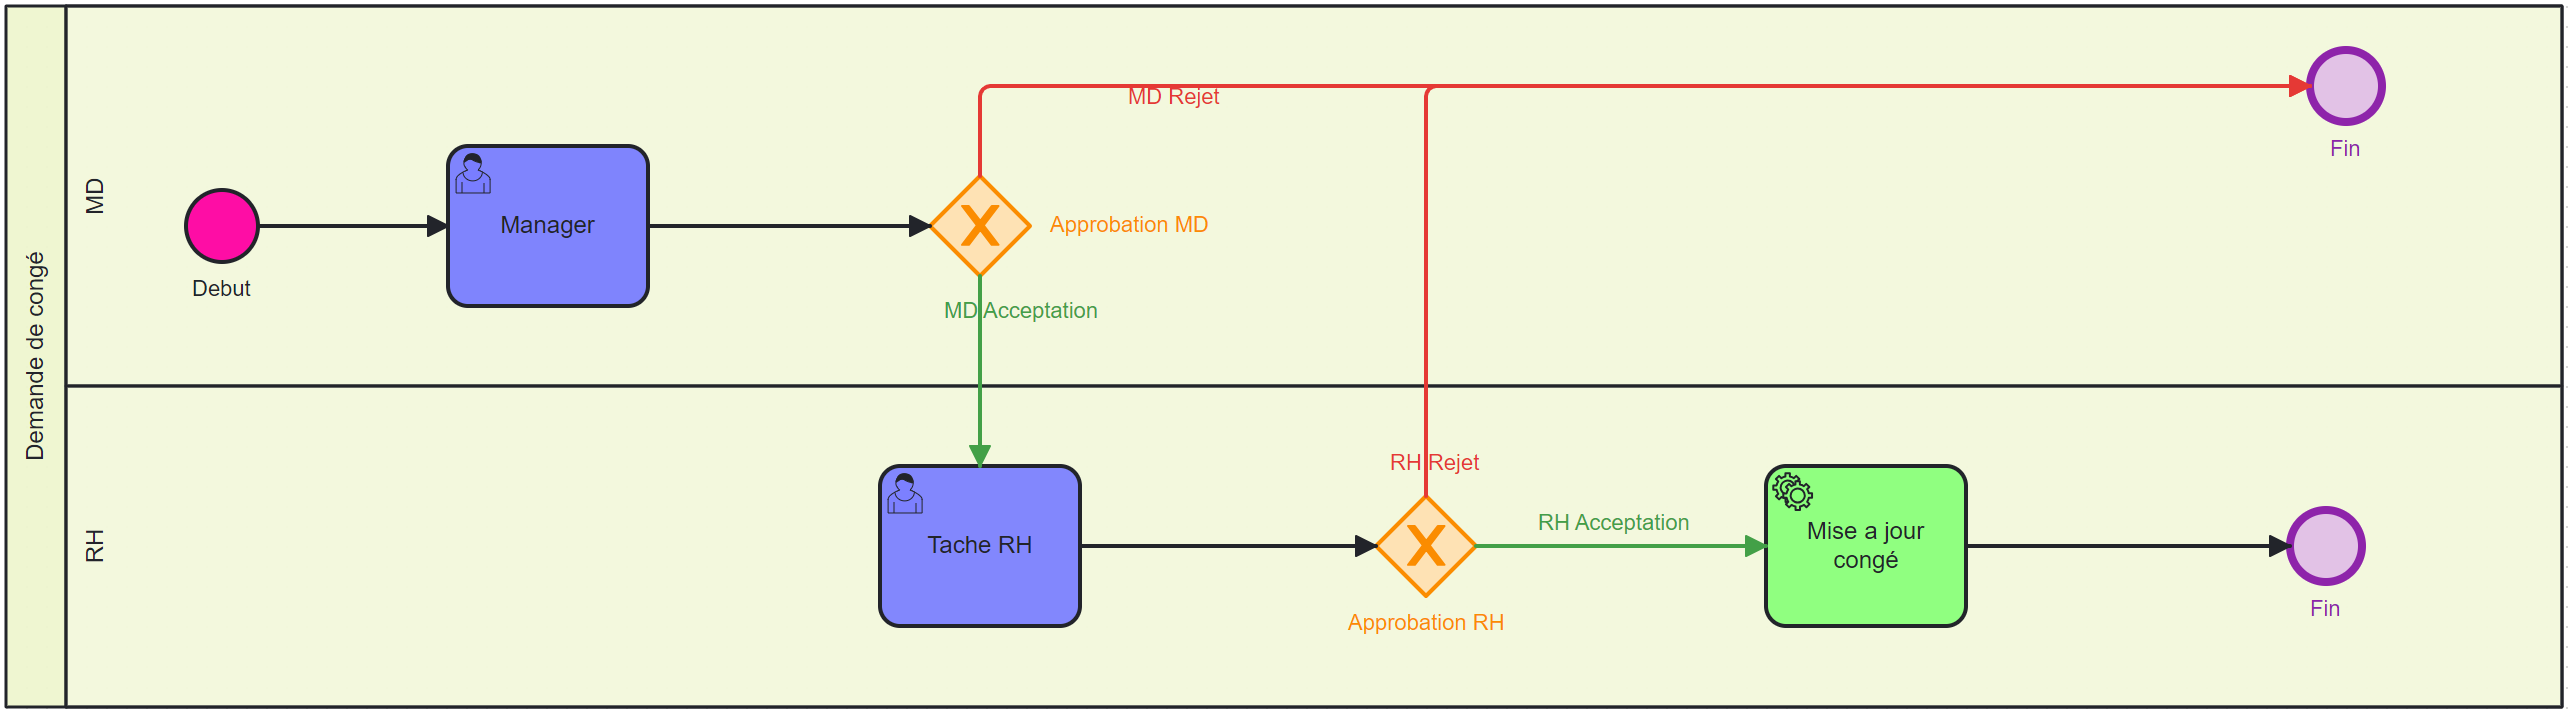
\includegraphics[width=17cm]{images/bpmn.png}
     \caption{Diagramme BPMN demande de congé}
     \label{fig:bpmnConge}
\end{figure}
\paragraph{Demande d’autorisation :}
Le processus débute par un événement de départ (\textbf{Début}).
Ensuite, une tâche utilisateur intitulée \textbf{Demande autorisation} est initiée, dans laquelle un utilisateur soumet une requête d'autorisation.

Un \textbf{gateway exclusif} (losange avec croix) permet de rediriger le processus selon le résultat de la demande :

Si la demande est refusée (chemin rouge), le processus se termine immédiatement par un événement de fin. 

Si la demande est approuvée (chemin vert), une tâche de service \textbf{Update autorisation} est exécutée.
Celle-ci permet de mettre à jour les informations d’autorisation dans le système.
Le processus se termine ensuite par un événement de fin classique.

Ce processus est typiquement orchestré par un moteur BPM tel que \textbf{Camunda}, permettant d’associer automatiquement des règles métiers et des traitements conditionnels à chaque étape. L'utilisation du gateway permet de gérer de façon claire et contrôlée les différentes issues de la demande.
\begin{figure}[h]
     \centering
     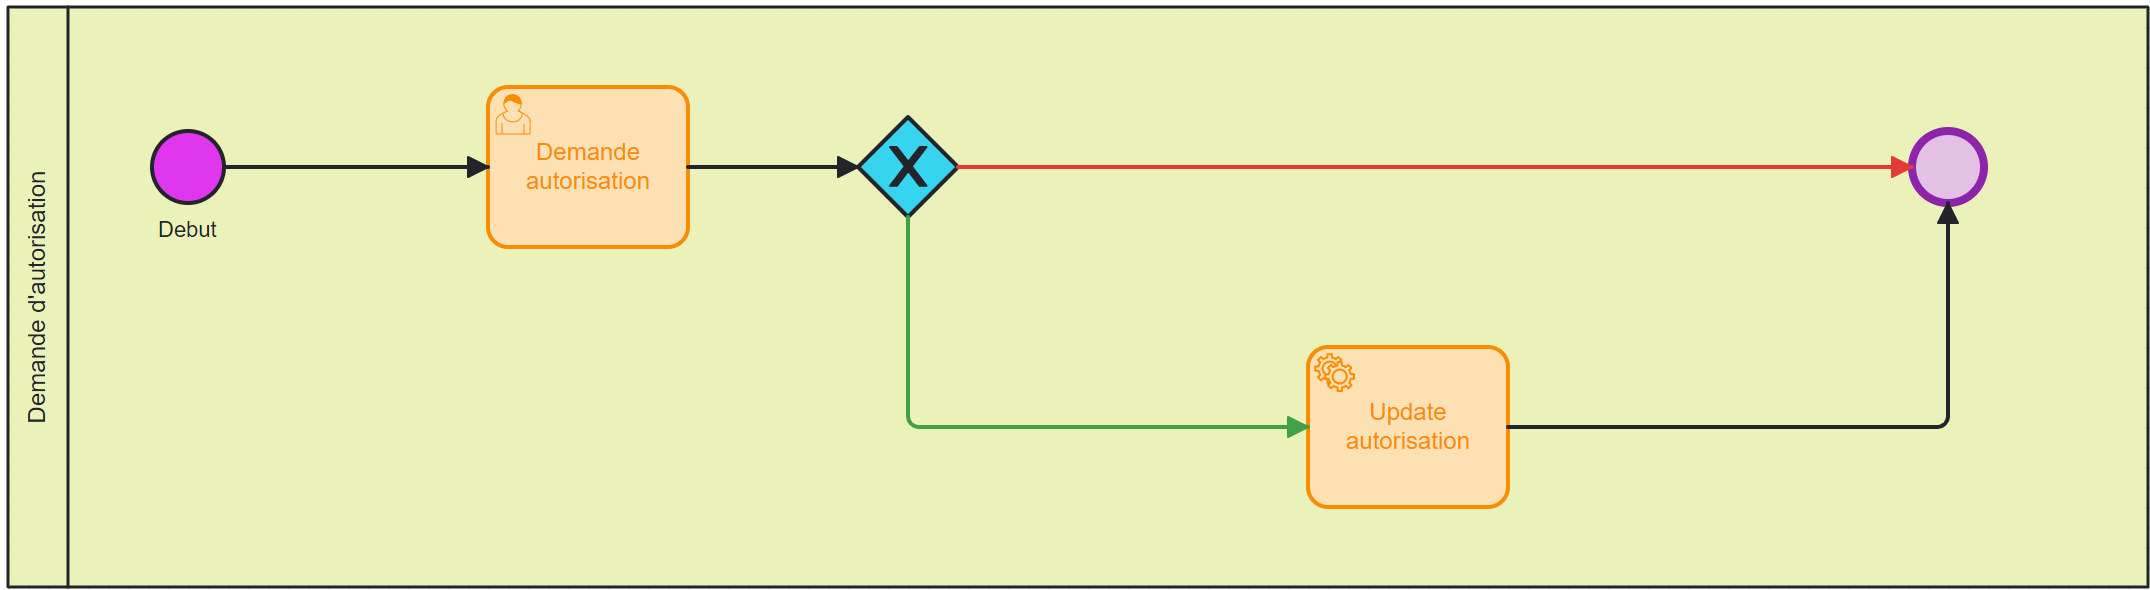
\includegraphics[width=17cm]{images/bpmn2.png}
     \caption{Diagramme BPMN demande d'autorisation}
     \label{fig:bpmnConge2}
\end{figure}
\newpage
\subsection{Conception du Cas d'Utilisation «Consulter ses demandes»}
\subsubsection{Diagramme de Classe}
La figure~\ref{fig:Consulter_ses_demandes} illustre le diagramme de classes du cas d'utilisation « Consulter ses demandes ».
\begin{figure}[h]
     \centering
     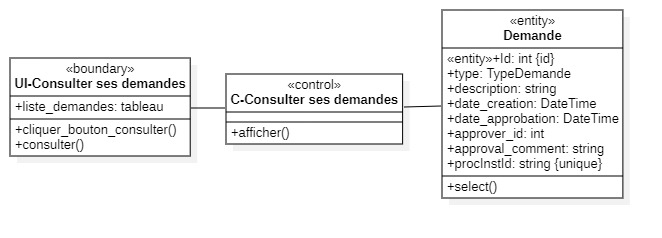
\includegraphics[width=15cm]{images/C-cdem.jpg}
     \caption{Diagramme de classe du cas d'utilisation <<Consulter ses demandes>>}
     \label{fig:Consulter_ses_demandes}
\end{figure}
\subsection{Diagramme de Séquence}
Les utilisateurs, les managers et les RH ont la possibilité de consulter leurs demandes à partir de leurs interfaces respectives. Les actions qu’ils réalisent pour consulter leurs demandes sont exécutées suite à la communication entre l’interface utilisateur et le contrôleur de consultation, qui interagit avec l’entité "Demande" pour récupérer les informations correspondantes depuis la base de données. Ce scénario est présenté dans la figure \ref{fig:S_Consulter_ses_demandes}.
\begin{figure}[h]
     \centering
     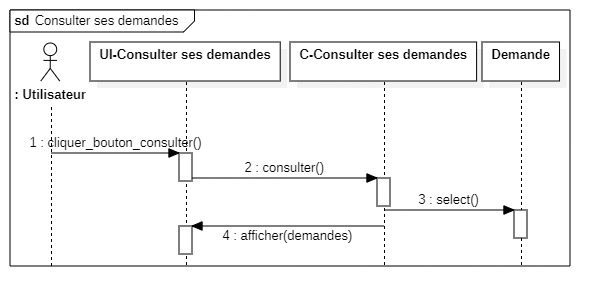
\includegraphics[width=15cm]{images/S-cdem.jpg}
     \caption{Diagramme de séquence du cas d'utilisation <<Consulter ses demandes>>}
     \label{fig:S_Consulter_ses_demandes}
\end{figure}
\newpage
\subsection{Conception du Cas d'Utilisation «Consulter ses congés»}
\subsubsection{Diagramme de Classe}
La figure~\ref{fig:Consulter_ses_conges} illustre le diagramme de classes du cas d'utilisation « Consulter ses congés ».
\begin{figure}[h]
     \centering
     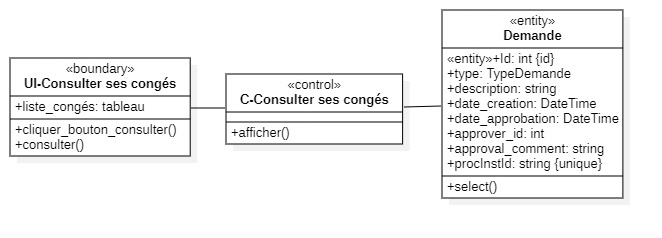
\includegraphics[width=15cm]{images/C-ccon.jpg}
     \vspace{-1cm}
     \caption{Diagramme de classe du cas d'utilisation <<Consulter ses congés>>}
     \label{fig:Consulter_ses_conges}
\end{figure}

\subsubsection{Diagramme de Séquence}
Les utilisateurs, les managers et les RH ont la possibilité de consulter leurs congés à partir de leurs interfaces respectives. Les actions qu'ils réalisent pour consulter leurs congés sont exécutées suite à la communication entre l'interface utilisateur et le contrôleur de consultation, qui interagit avec l'entité "Demande" pour récupérer les informations correspondantes depuis la base de données(Les demandes approuvées). Ce scénario est présenté dans la figure \ref{fig:S_Consulter_ses_conges}.
\begin{figure}[h]
     \centering
     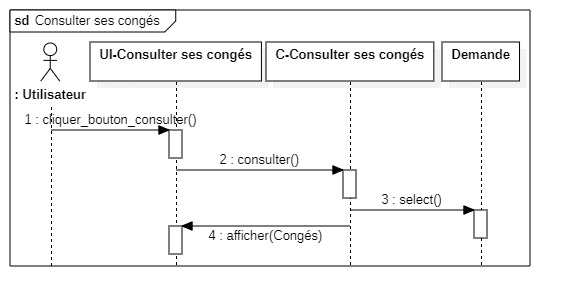
\includegraphics[width=15cm]{images/S-ccon.jpg}
     \caption{Diagramme de séquence du cas d'utilisation <<Consulter ses congés>>}
     \label{fig:S_Consulter_ses_conges}
\end{figure}
\newpage
\subsection{Conception du Cas d'Utilisation «Traiter une demande»}

\subsubsection{Diagramme de Classe}
La figure~\ref{fig:Traiter_demande_classe} illustre le diagramme de classes du cas d'utilisation « Traiter une demande ».

\begin{figure}[h]
     \centering
     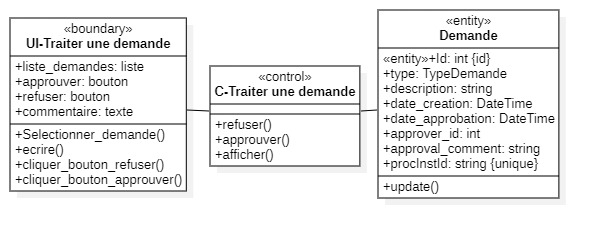
\includegraphics[width=15cm]{images/C-tdem.jpg}
     \caption{Diagramme de classe du cas d'utilisation <<Traiter une demande>>}
     \label{fig:Traiter_demande_classe}
\end{figure}

\subsubsection{Diagramme de Séquence}
Les managers et les responsables RH ont la possibilité de traiter les demandes qui leur sont adressées. Lors du traitement d'une demande, le manager doit d'abord approuver ou rejeter la demande. Si le manager rejette, la demande est automatiquement refusée. Si le manager approuve, la demande est transmise au responsable RH qui, à son tour, doit également approuver ou rejeter. Si le responsable RH rejette, la demande est refusée ; sinon, elle est approuvée. Ce scénario est illustré dans la figure~\ref{fig:Traiter_demande_sequence}.
\clearpage
\begin{figure}[!h]
     \centering
     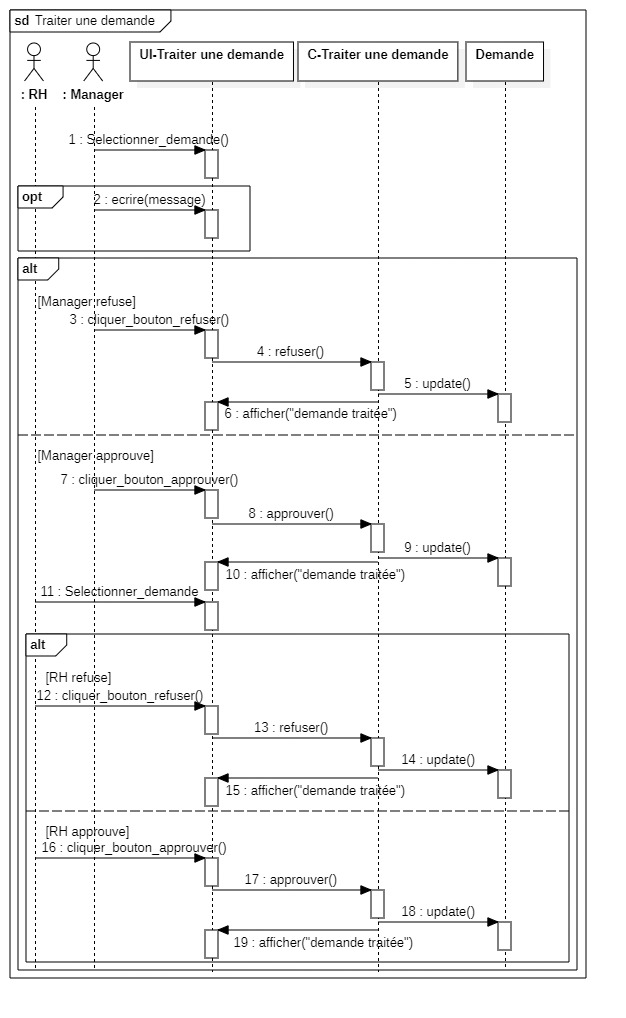
\includegraphics[width=15cm]{images/S-tdem.jpg}
     \vspace{-0.5cm}
     \caption{Diagramme de séquence du cas d'utilisation <<Traiter une demande>>}
     \label{fig:Traiter_demande_sequence}
\end{figure}
\clearpage
\section{Réalisation}
Dans cette partie, nous présentons les modules de notre premier sprint en utilisant des captures d’écran.
\subsection{Gérer son profil}
L'interface de gestion du profil présentée dans la figure \ref{fig:gp} permet aux utilisateurs de consulter et de modifier leurs informations personnelles. Ils ont la possibilité de mettre à jour leur photo de profil, ainsi que de corriger leur nom et prénom en cas d'erreur. Cette fonctionnalité garantit que les données utilisateur restent exactes et à jour, offrant ainsi une expérience personnalisée et fiable.
\begin{figure}[h]
     \centering
     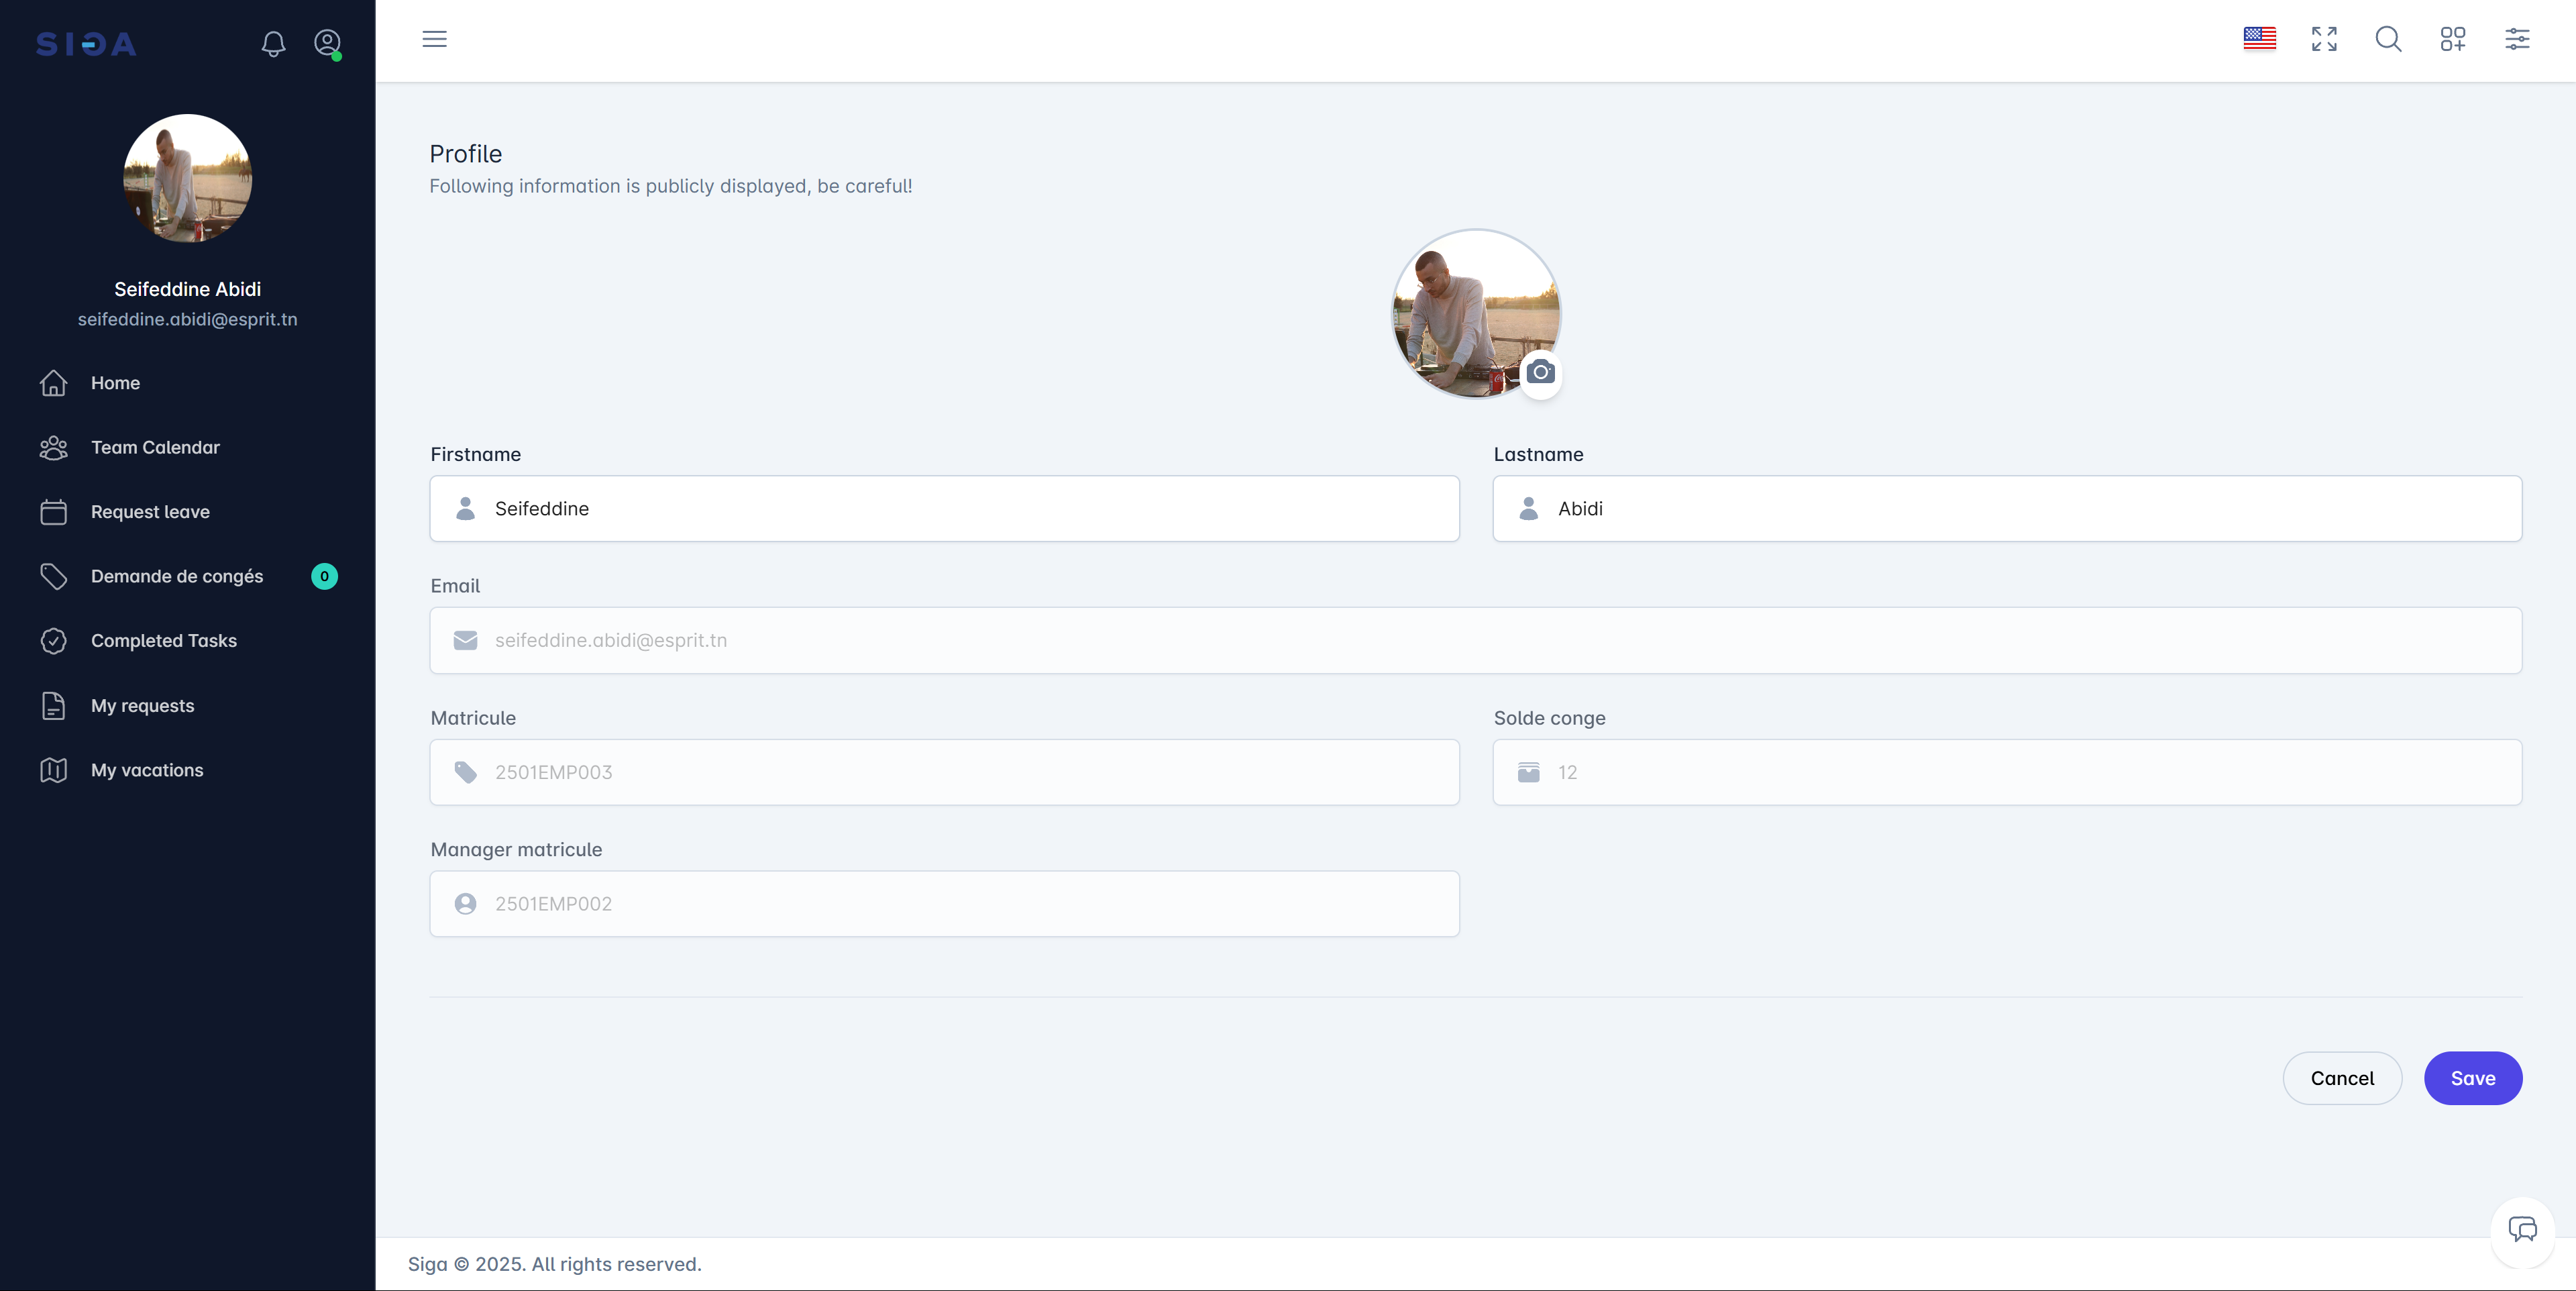
\includegraphics[width=16cm]{images/realisation/gp.png}
     \caption{Interface du cas d’utilisation «Gérer son profil»}
     \label{fig:gp}
\end{figure}
\subsection{Réinitialiser son mot de passe}
Pour réinitialiser le mot de passe, on doit suivre ces étapes :
\begin{enumerate}
    \item \textbf{Accédez à la page "Mot de passe oublié ?"} : Depuis la page de connexion, cliquez sur "Forgot password?".
    \item \textbf{Entrez votre adresse e-mail} : Saisissez l'adresse e-mail associée à votre compte dans le champ prévu ("Email address").
    \item \textbf{Envoyez la demande} : Cliquez sur le bouton "Send reset link". Un message confirmera l'envoi d'un e-mail si votre adresse est enregistrée dans le système.
    \item \textbf{Consultez votre boîte de réception} : Vous recevrez un e-mail intitulé "Password Reset Request" avec un bouton "Reset Password". Cliquez sur ce bouton.
    \newpage
    \vspace*{-2cm}
    \item \textbf{Créez un nouveau mot de passe} : Sur la page de réinitialisation, entrez votre e-mail, un nouveau mot de passe, et confirmez ce mot de passe dans les champs correspondants.
    \item \textbf{Validez} : Cliquez sur "Reset your password" pour enregistrer votre nouveau mot de passe.
\end{enumerate}
\begin{figure}[h]
    \centering
    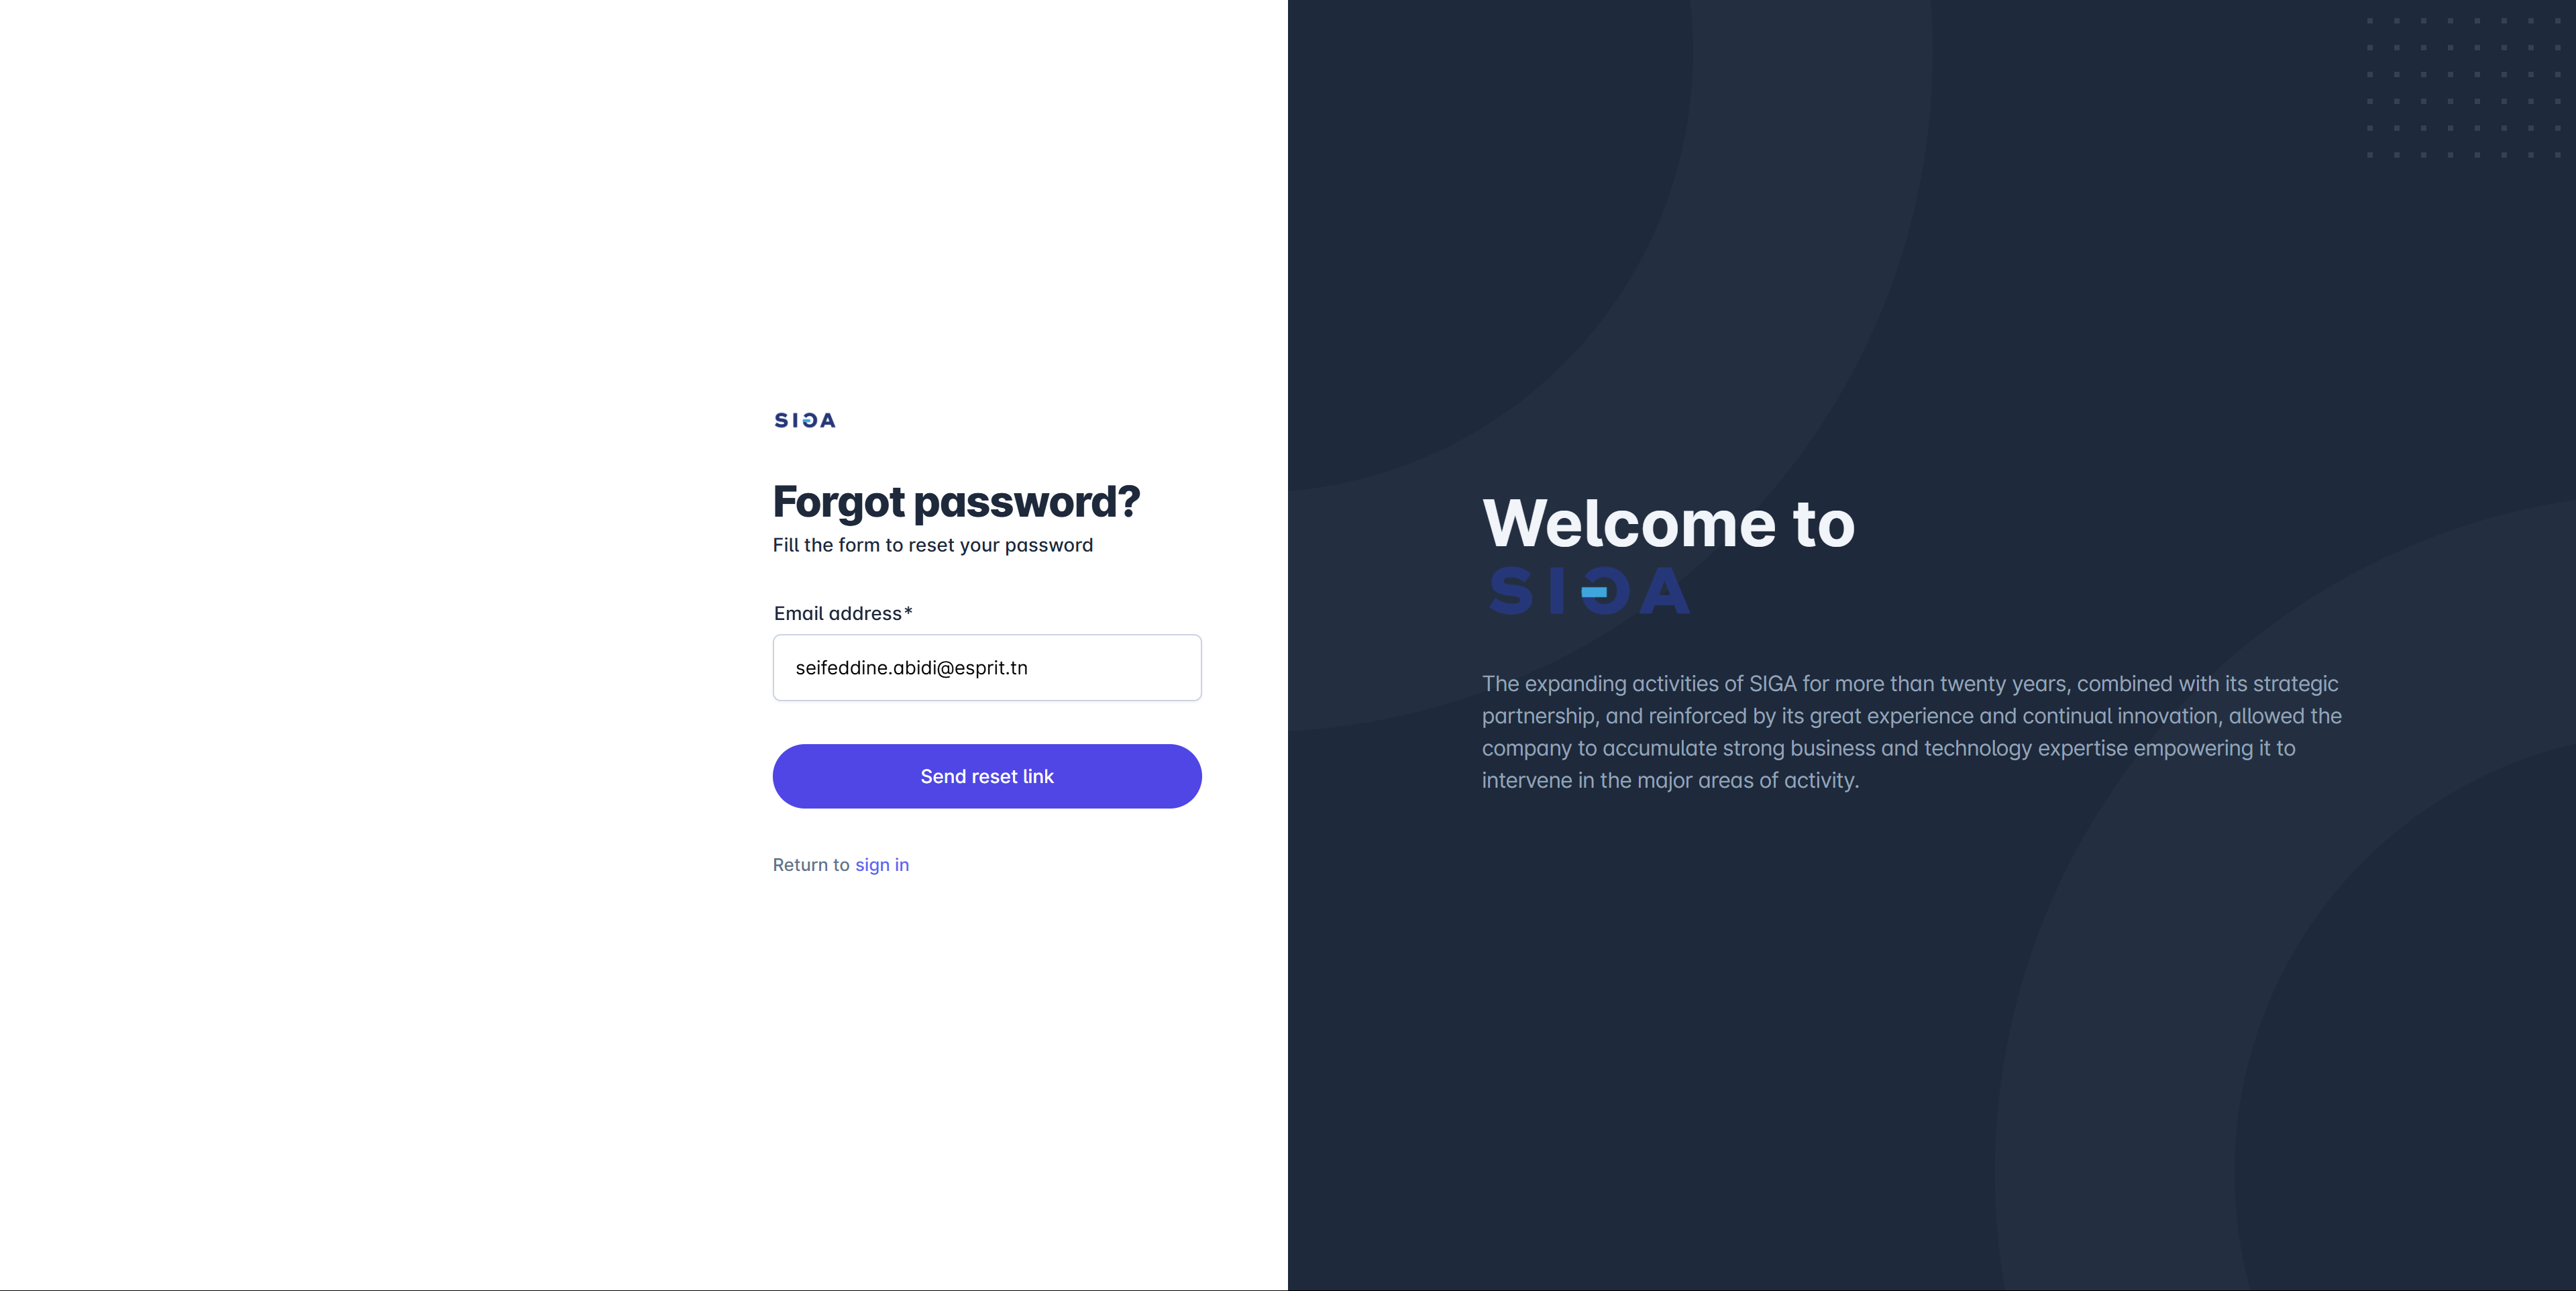
\includegraphics[width=16cm]{images/realisation/reset1.png}
    \caption{Page "Mot de passe oublié ?"}
    \label{fig:forgot_password}
\end{figure}
\begin{figure}[!h]
\vspace{-1cm}
    \centering
    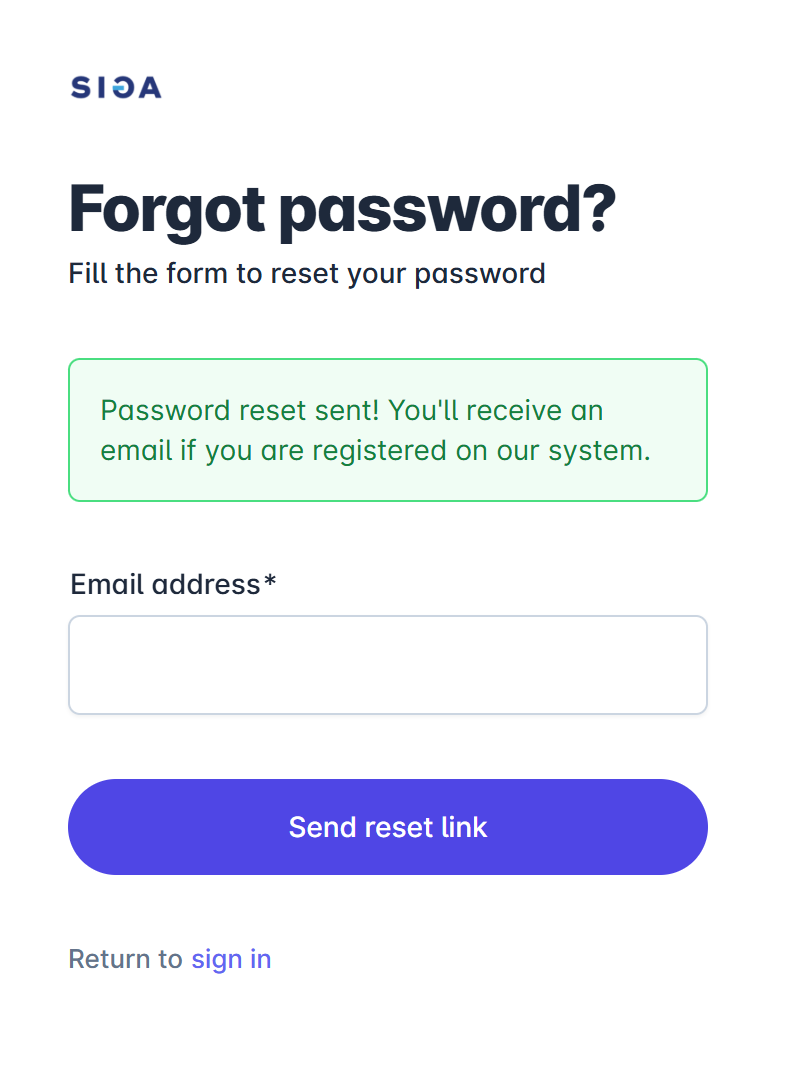
\includegraphics[width=6cm]{images/realisation/reset2.png}
    \caption{Confirmation de l'envoi du lien de réinitialisation}
    \label{fig:reset_success}
\end{figure}

\begin{figure}[h]
    \centering
    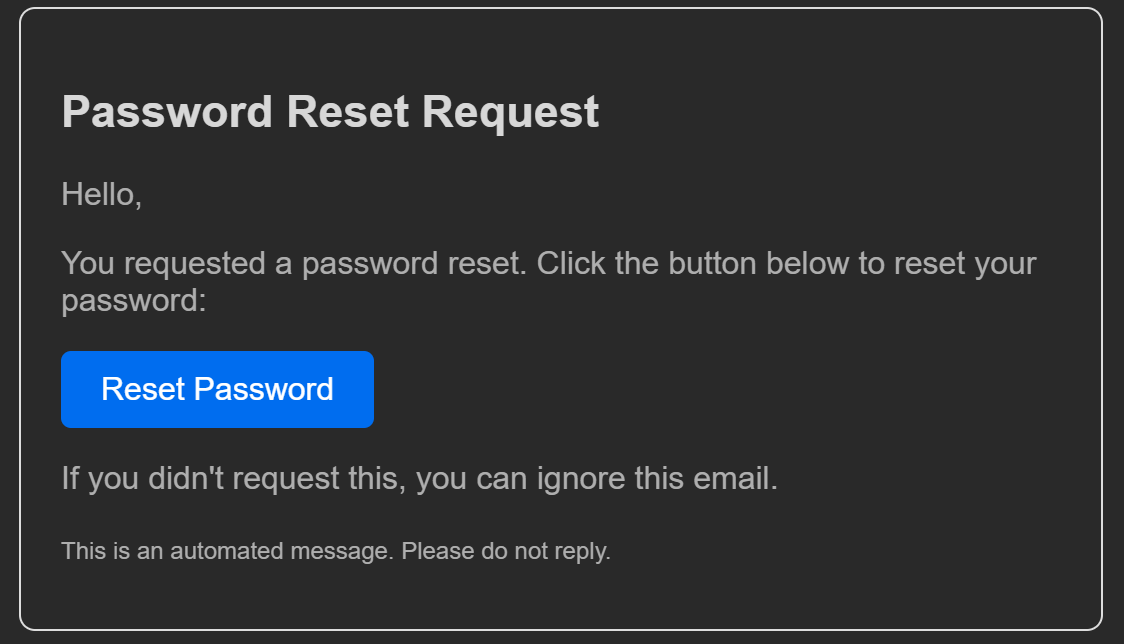
\includegraphics[width=16cm]{images/realisation/reset3.png}
    \caption{E-mail de réinitialisation de mot de passe}
    \label{fig:email_reset}
\end{figure}

\begin{figure}[h]
    \centering
    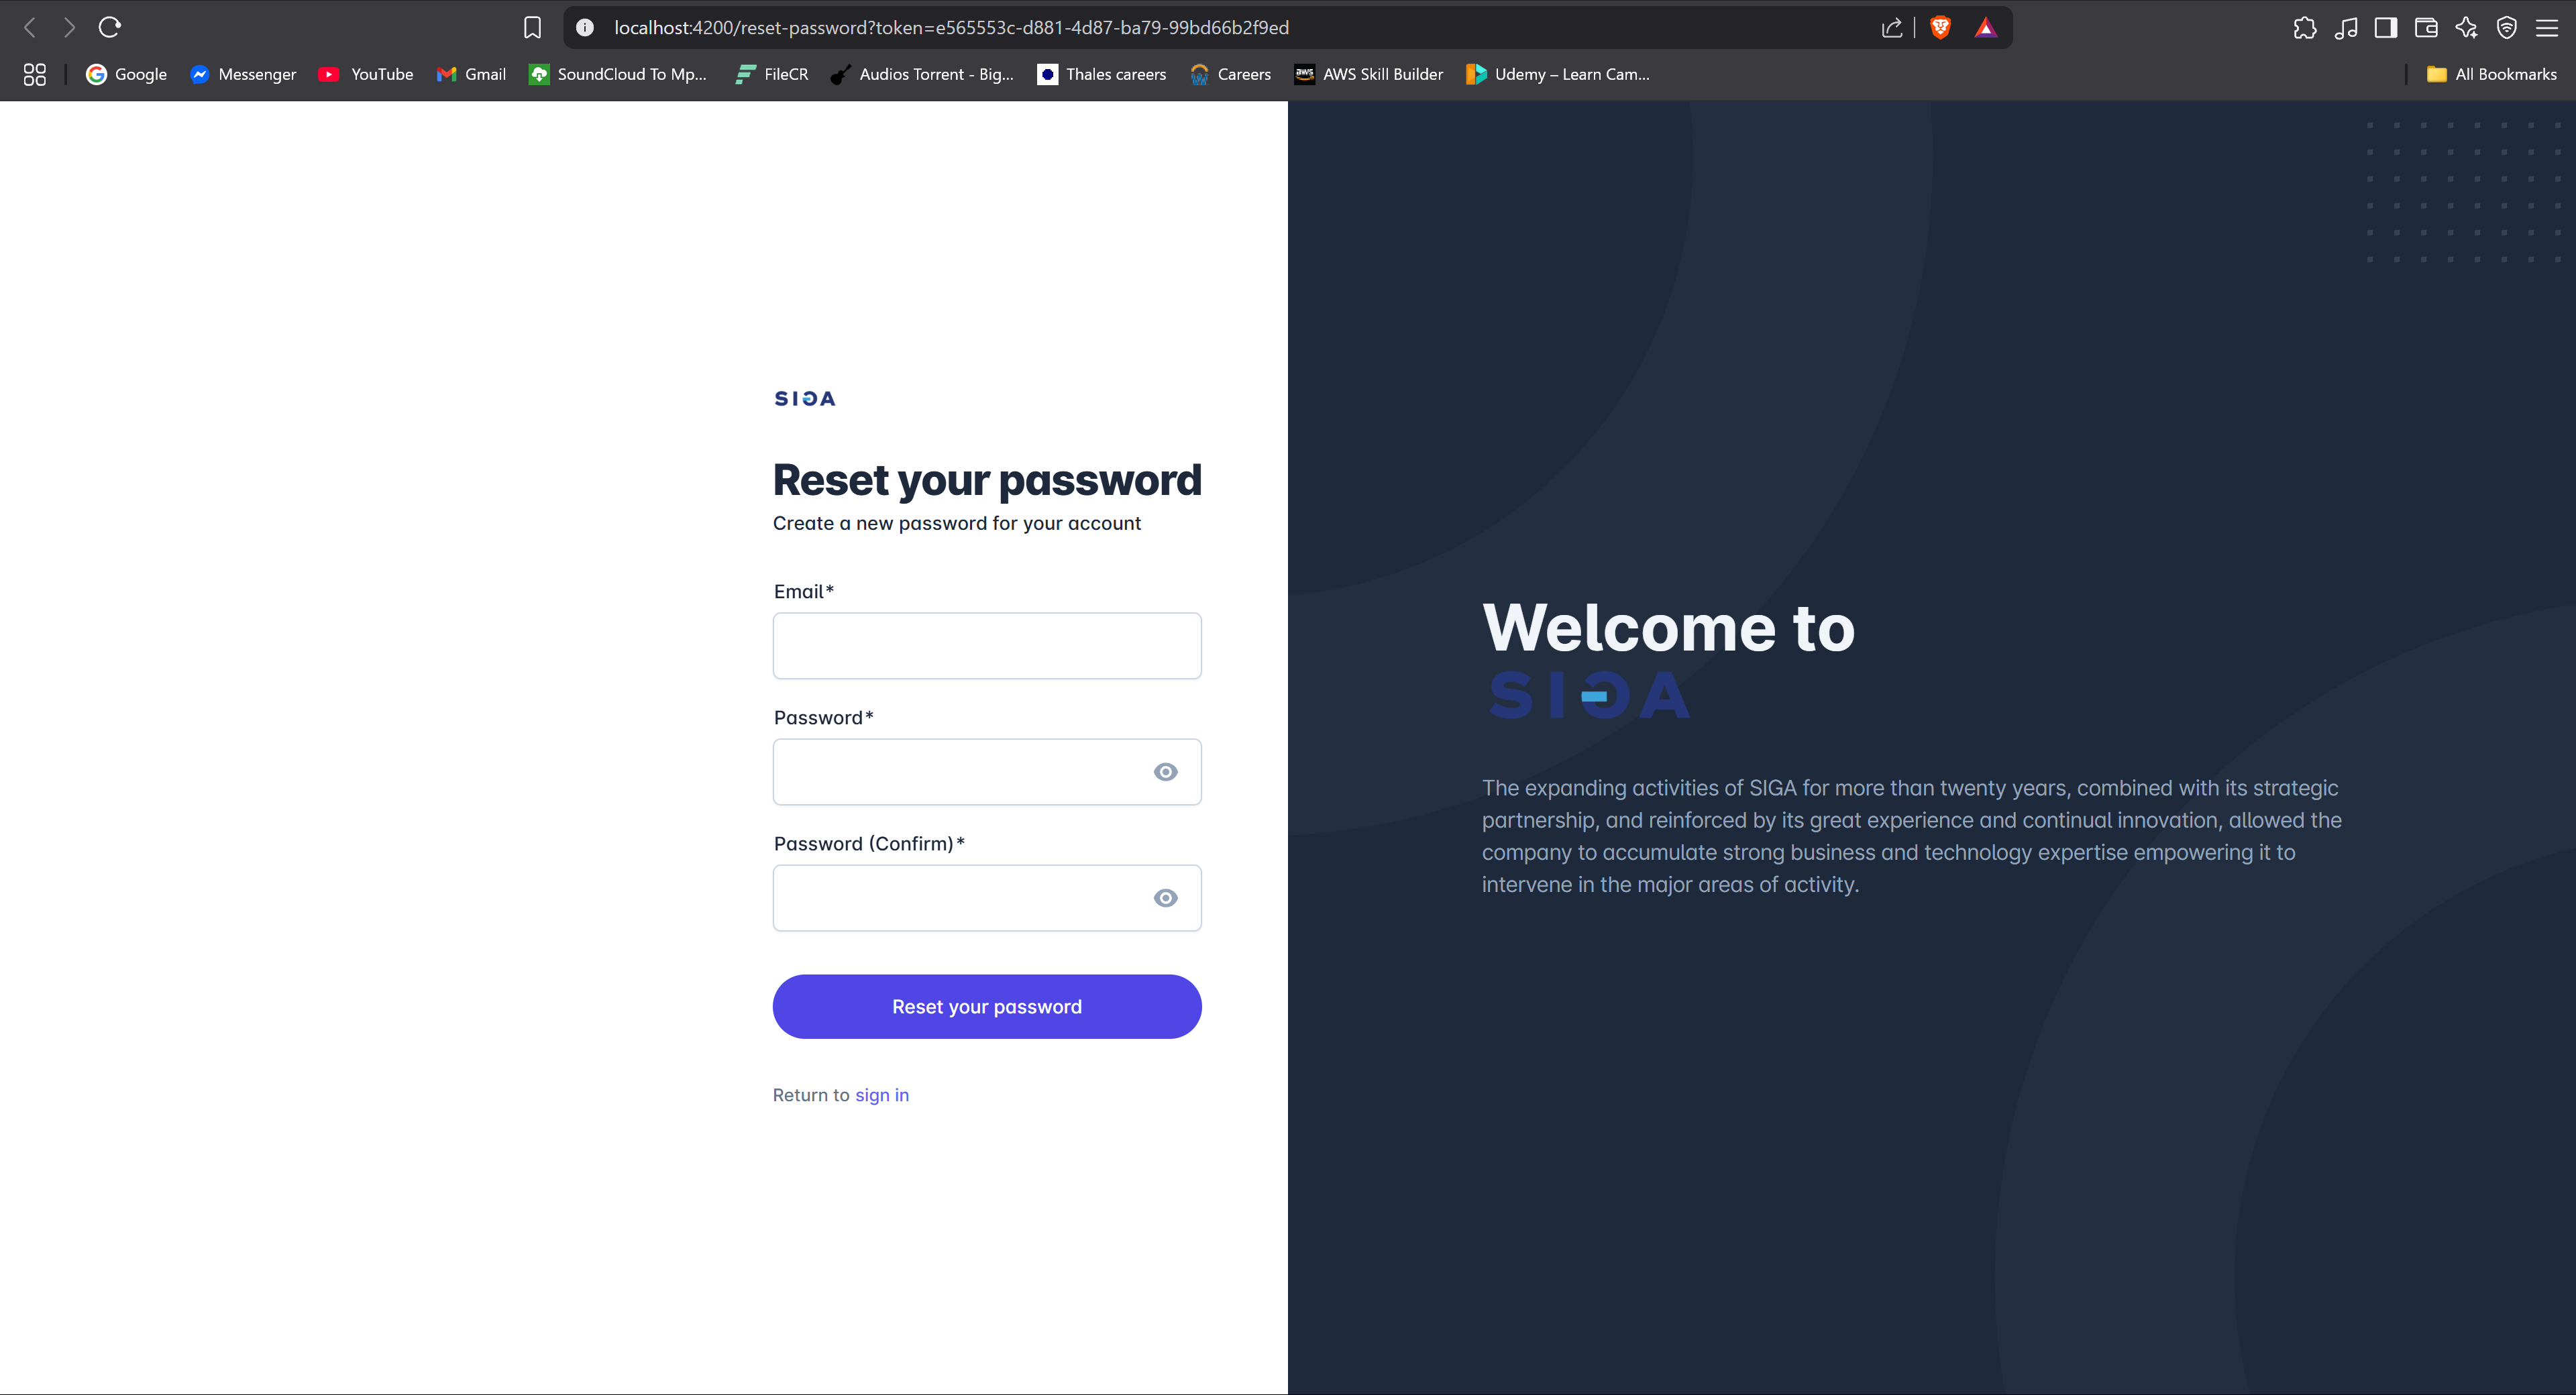
\includegraphics[width=16cm]{images/realisation/reset4.png}
    \caption{Page de création d'un nouveau mot de passe}
    \label{fig:reset_password}
\end{figure}
\clearpage
\subsection{Soumettre une demande}
\begin{enumerate}
    \item \textbf{Sélectionner le type de la demande} : Commencez par choisir le type de demande que vous souhaitez soumettre via un menu déroulant ou une liste (par exemple, "Leave request" pour une demande de congé comme illustré dans la figure \ref{fig:sund} et \ref{fig:sund2}).
    \item \textbf{Remplir les informations nécessaires} : Indiquez les détails requis, tels que les dates de début et de fin, ainsi que les horaires si pertinents.
    \item \textbf{Ajouter des options supplémentaires} : Si applicable, précisez des préférences ou conditions spécifiques (par exemple, un départ ou un retour en milieu de journée).
    \item \textbf{Soumettre la demande} : Une fois toutes les informations saisies, validez votre demande en cliquant sur un bouton de soumission. Vous pouvez également annuler si nécessaire.
\end{enumerate}
\begin{figure}[h]
    \centering
    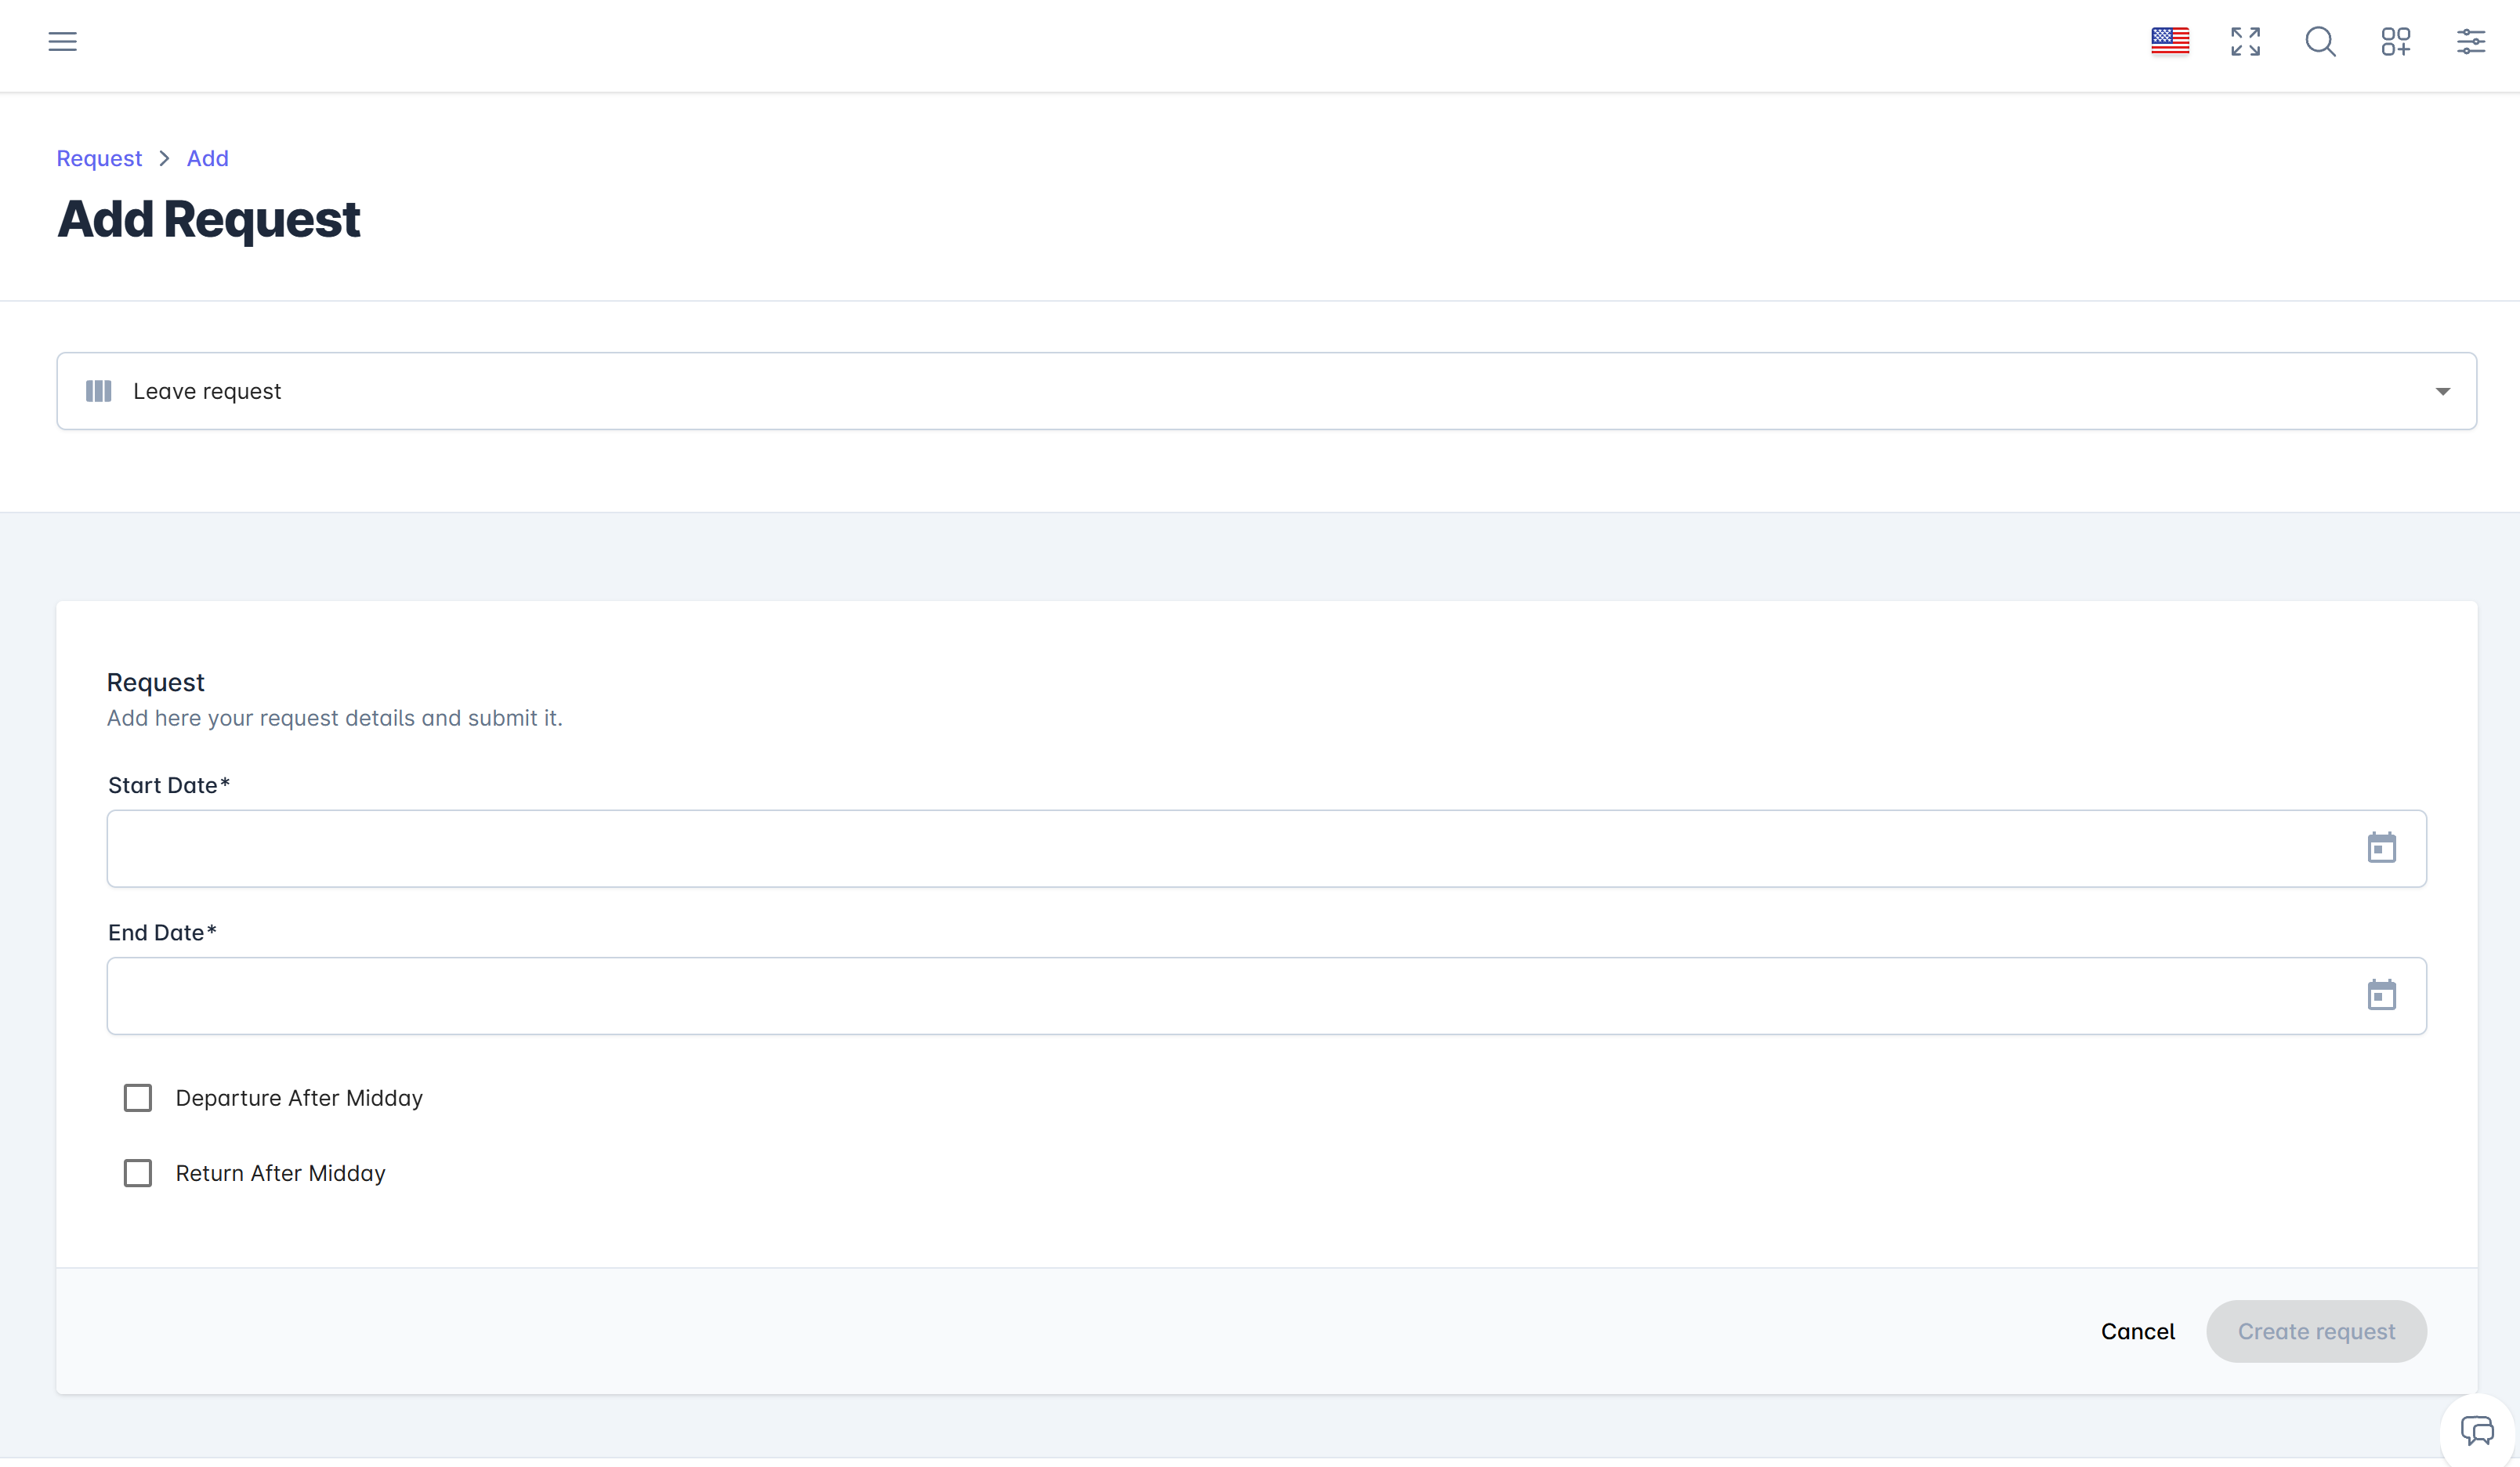
\includegraphics[width=16cm]{images/realisation/addReq.png}
    \caption{Page de création d'une nouvelle demande de congé}
    \label{fig:sund}
\end{figure}
\newpage
\begin{figure}[h]
\vspace{-2.2cm}
    \centering
    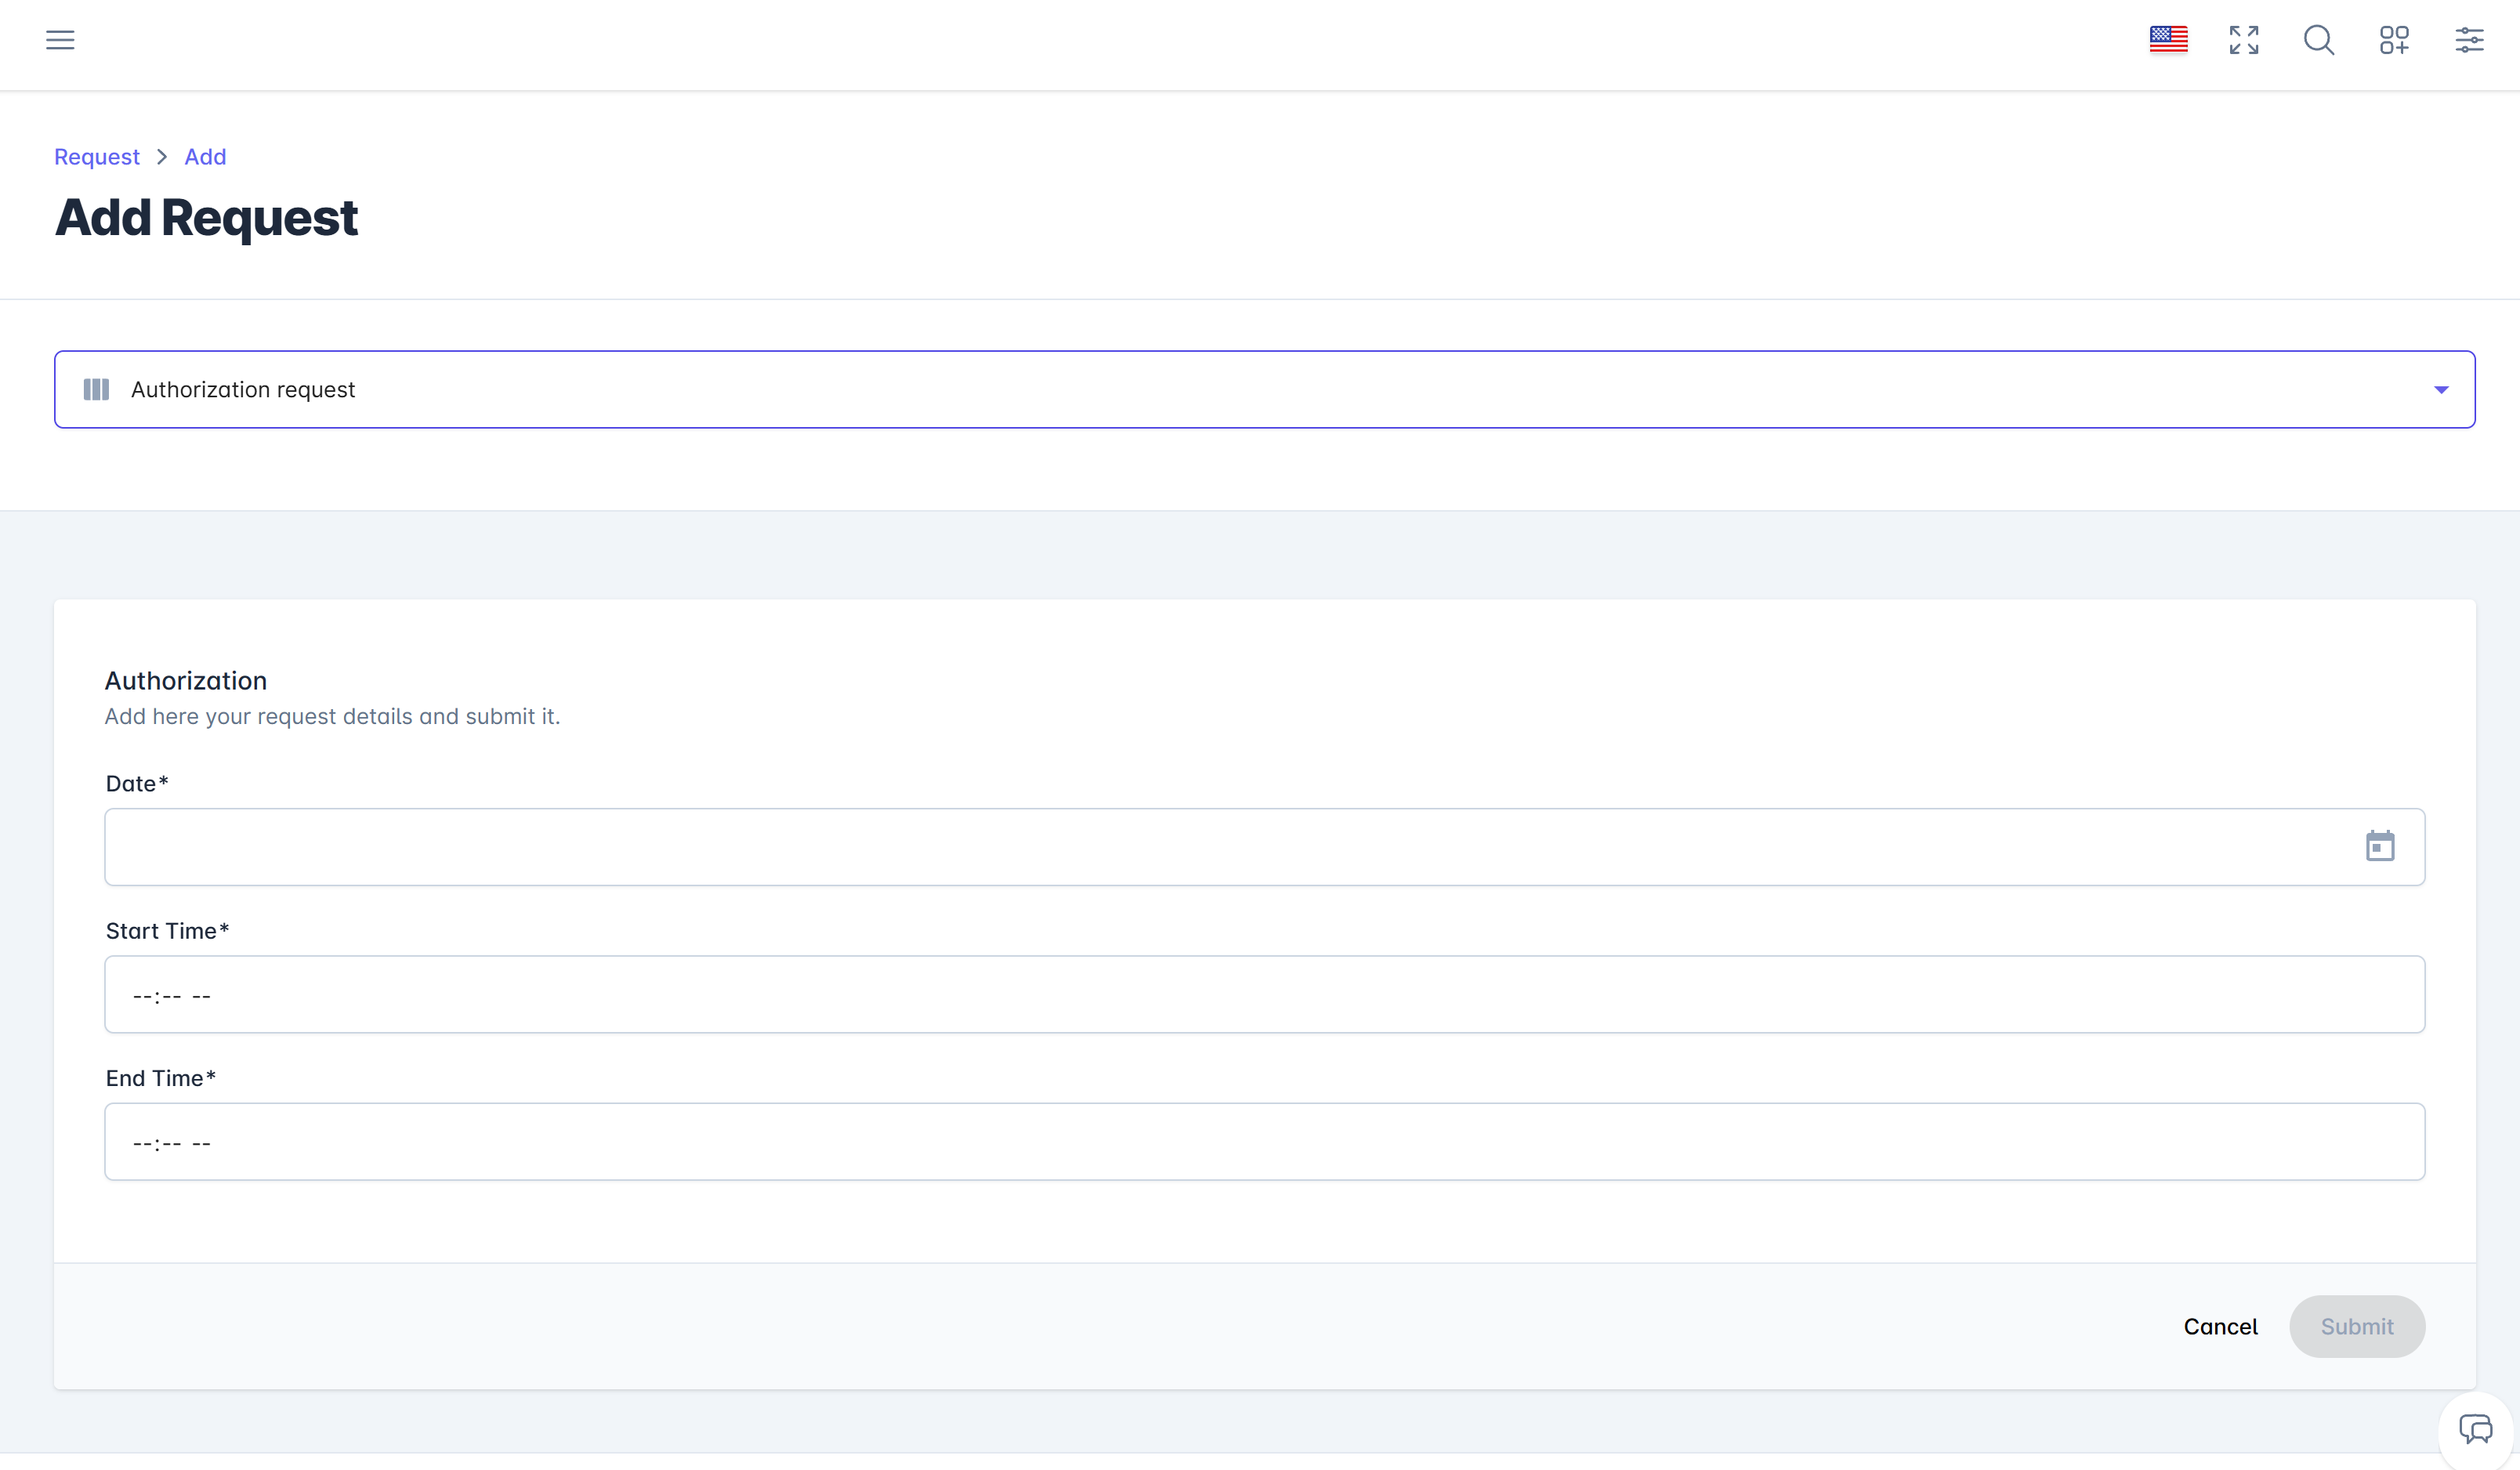
\includegraphics[width=16cm]{images/realisation/addReq2.png}
    \caption{Page de création d'un nouvelle demande d'autorisation}
    \label{fig:sund2}
\end{figure}
\subsection{Consulter ses demandes}
\begin{figure}[h]
\vspace{-0.6cm}
    \centering
    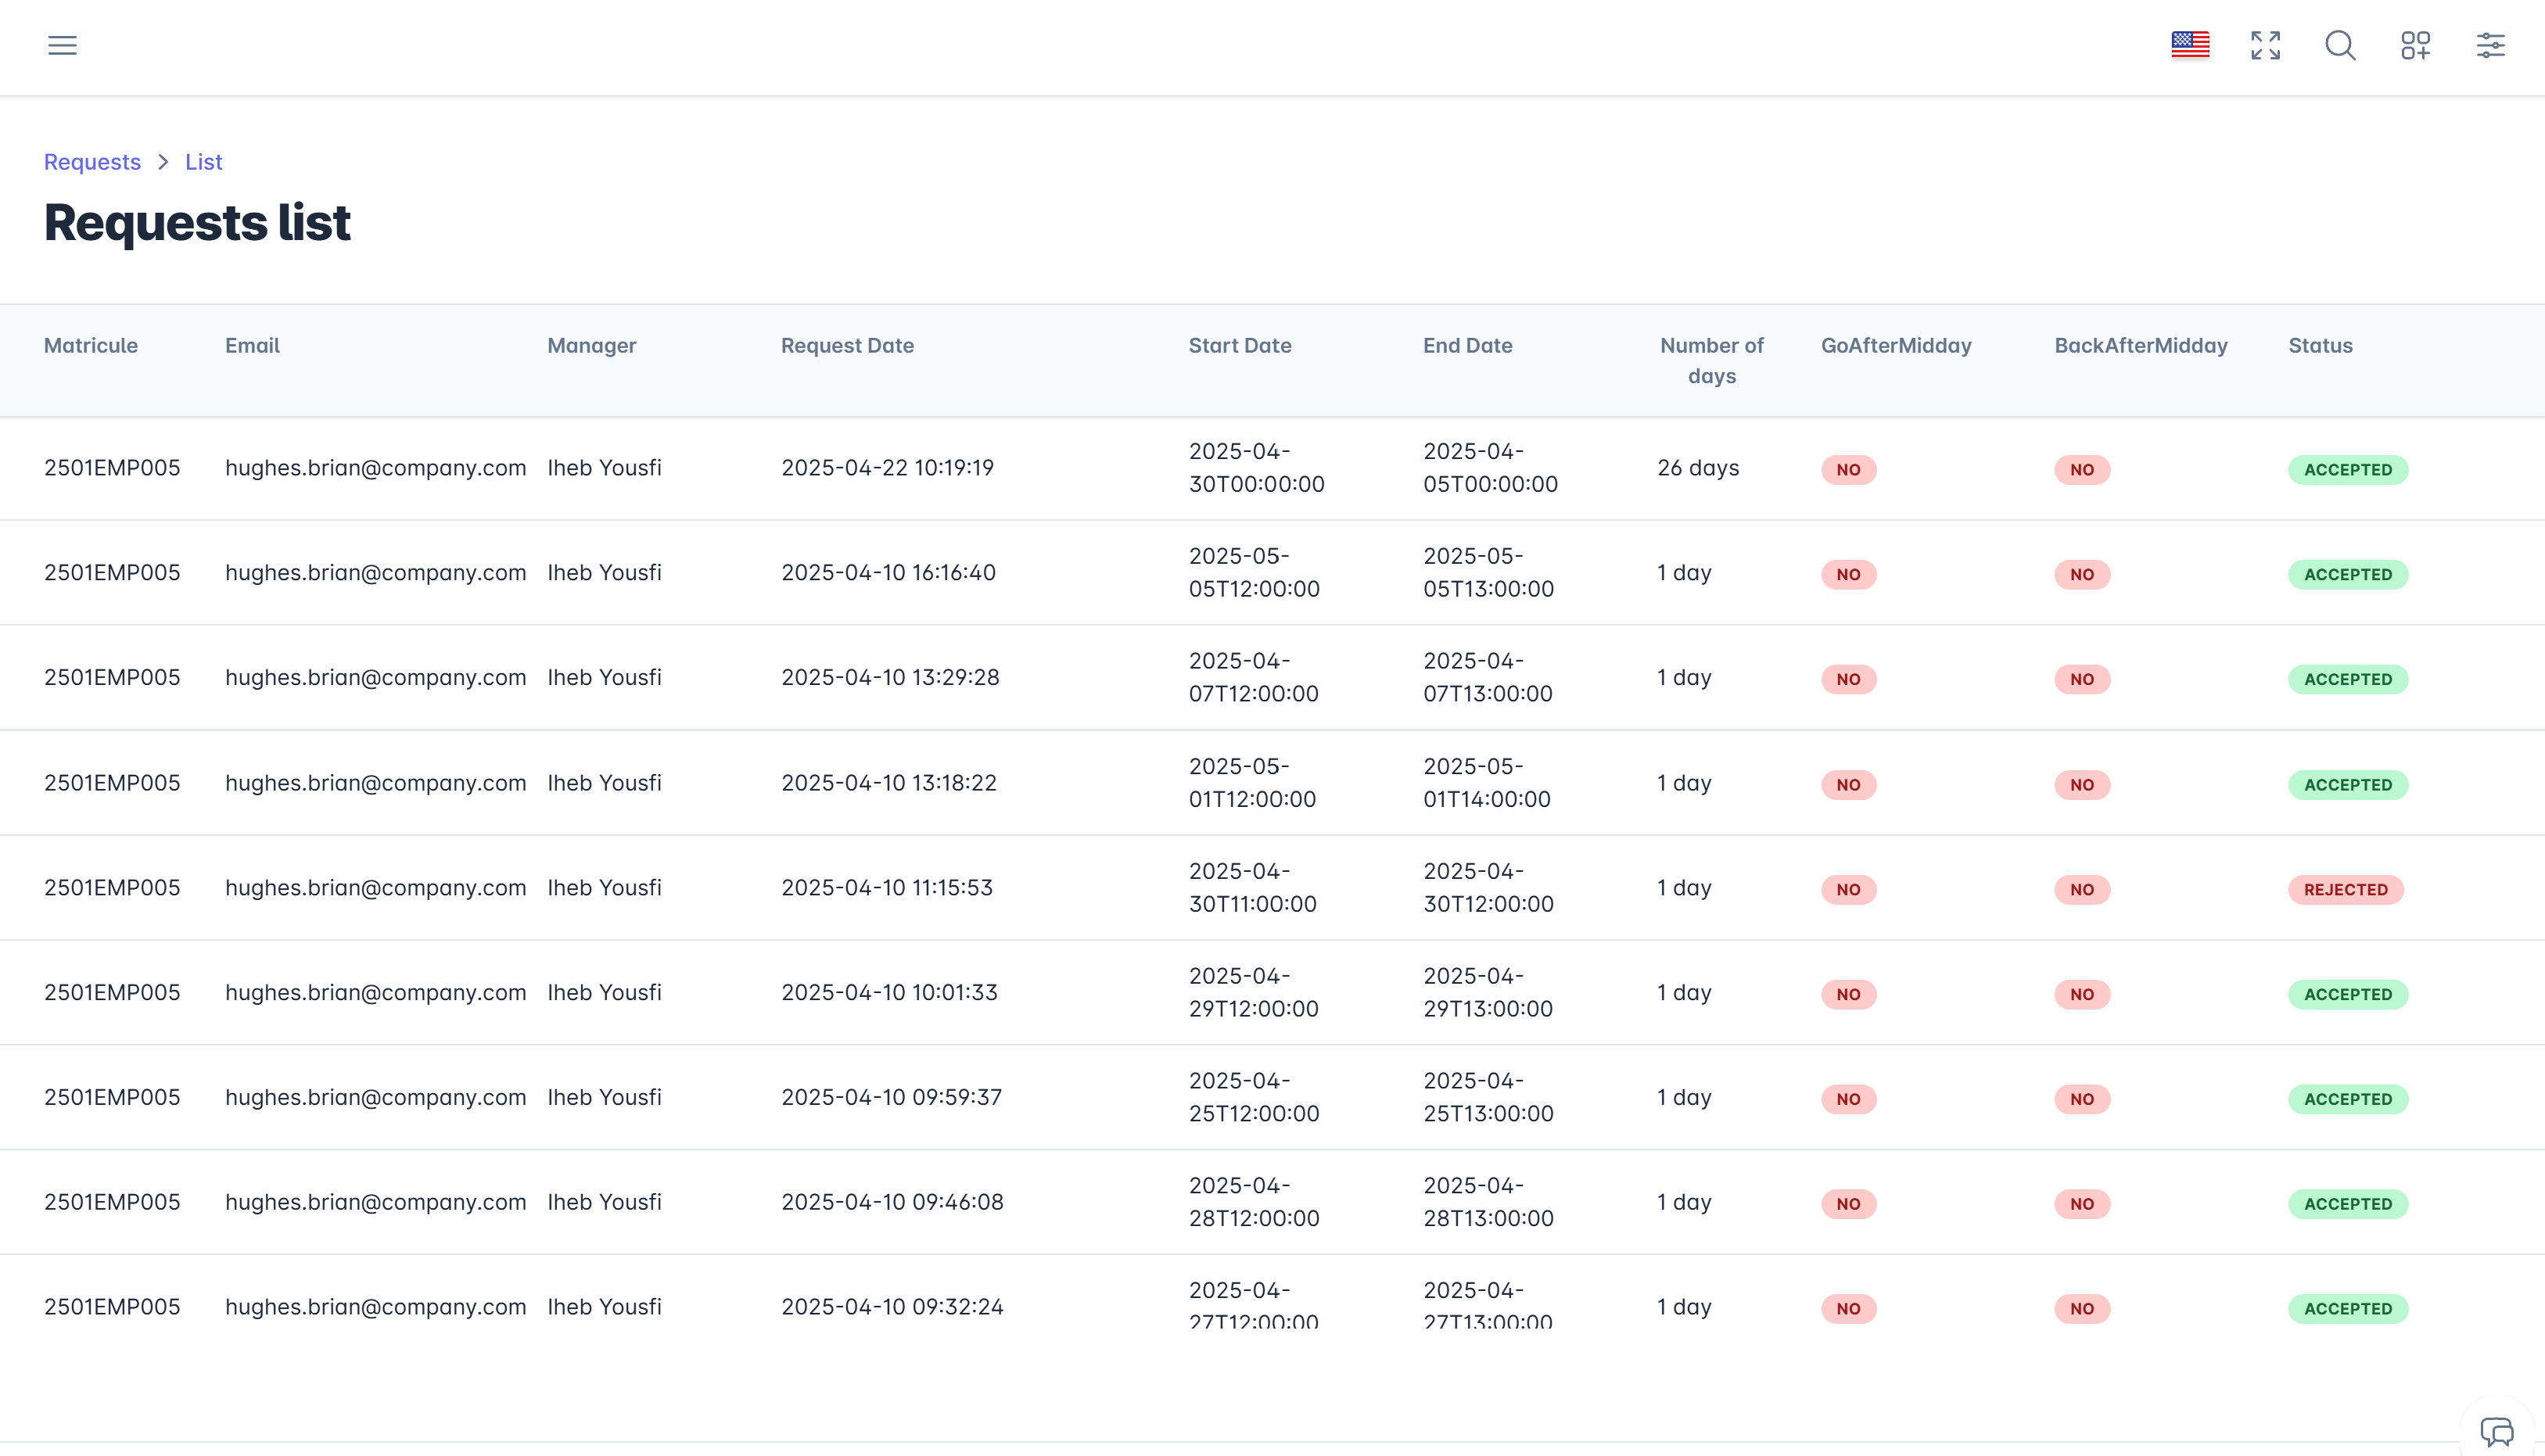
\includegraphics[width=15cm]{images/realisation/mesDemandes.png}
    \caption{Page de consultation des demandes personnelles}
    \label{fig:Cmesd}
\end{figure}
\newpage

L'interface pour consulter ses demandes sur une plateforme comme celle présentée est généralement conçue pour être intuitive et organisée. Une fois dans cette section, l'utilisateur voit une liste ou un tableau répertoriant ses demandes soumises. Chaque entrée affiche des informations clés telles que la date de soumission, les dates demandées (début et fin), et l'état de la demande (en attente, approuvée ou rejetée). Des options de tri peuvent être présentes, permettant de classer les demandes par statut ou par date.
\subsection{Consulter ses congés}
L'interface pour consulter ses congés, c'est-à-dire les demandes de congés qui ont été acceptées, est conçue pour fournir une vue organisée et spécifique des congés approuvés. Une fois dans cette section, l'utilisateur voit une liste ou un tableau répertoriant uniquement ses demandes de congés ayant été acceptées. Chaque entrée affiche des informations clés telles que les dates de début et de fin du congé, la date d'approbation, et éventuellement la durée.
\begin{figure}[h]
         \centering
         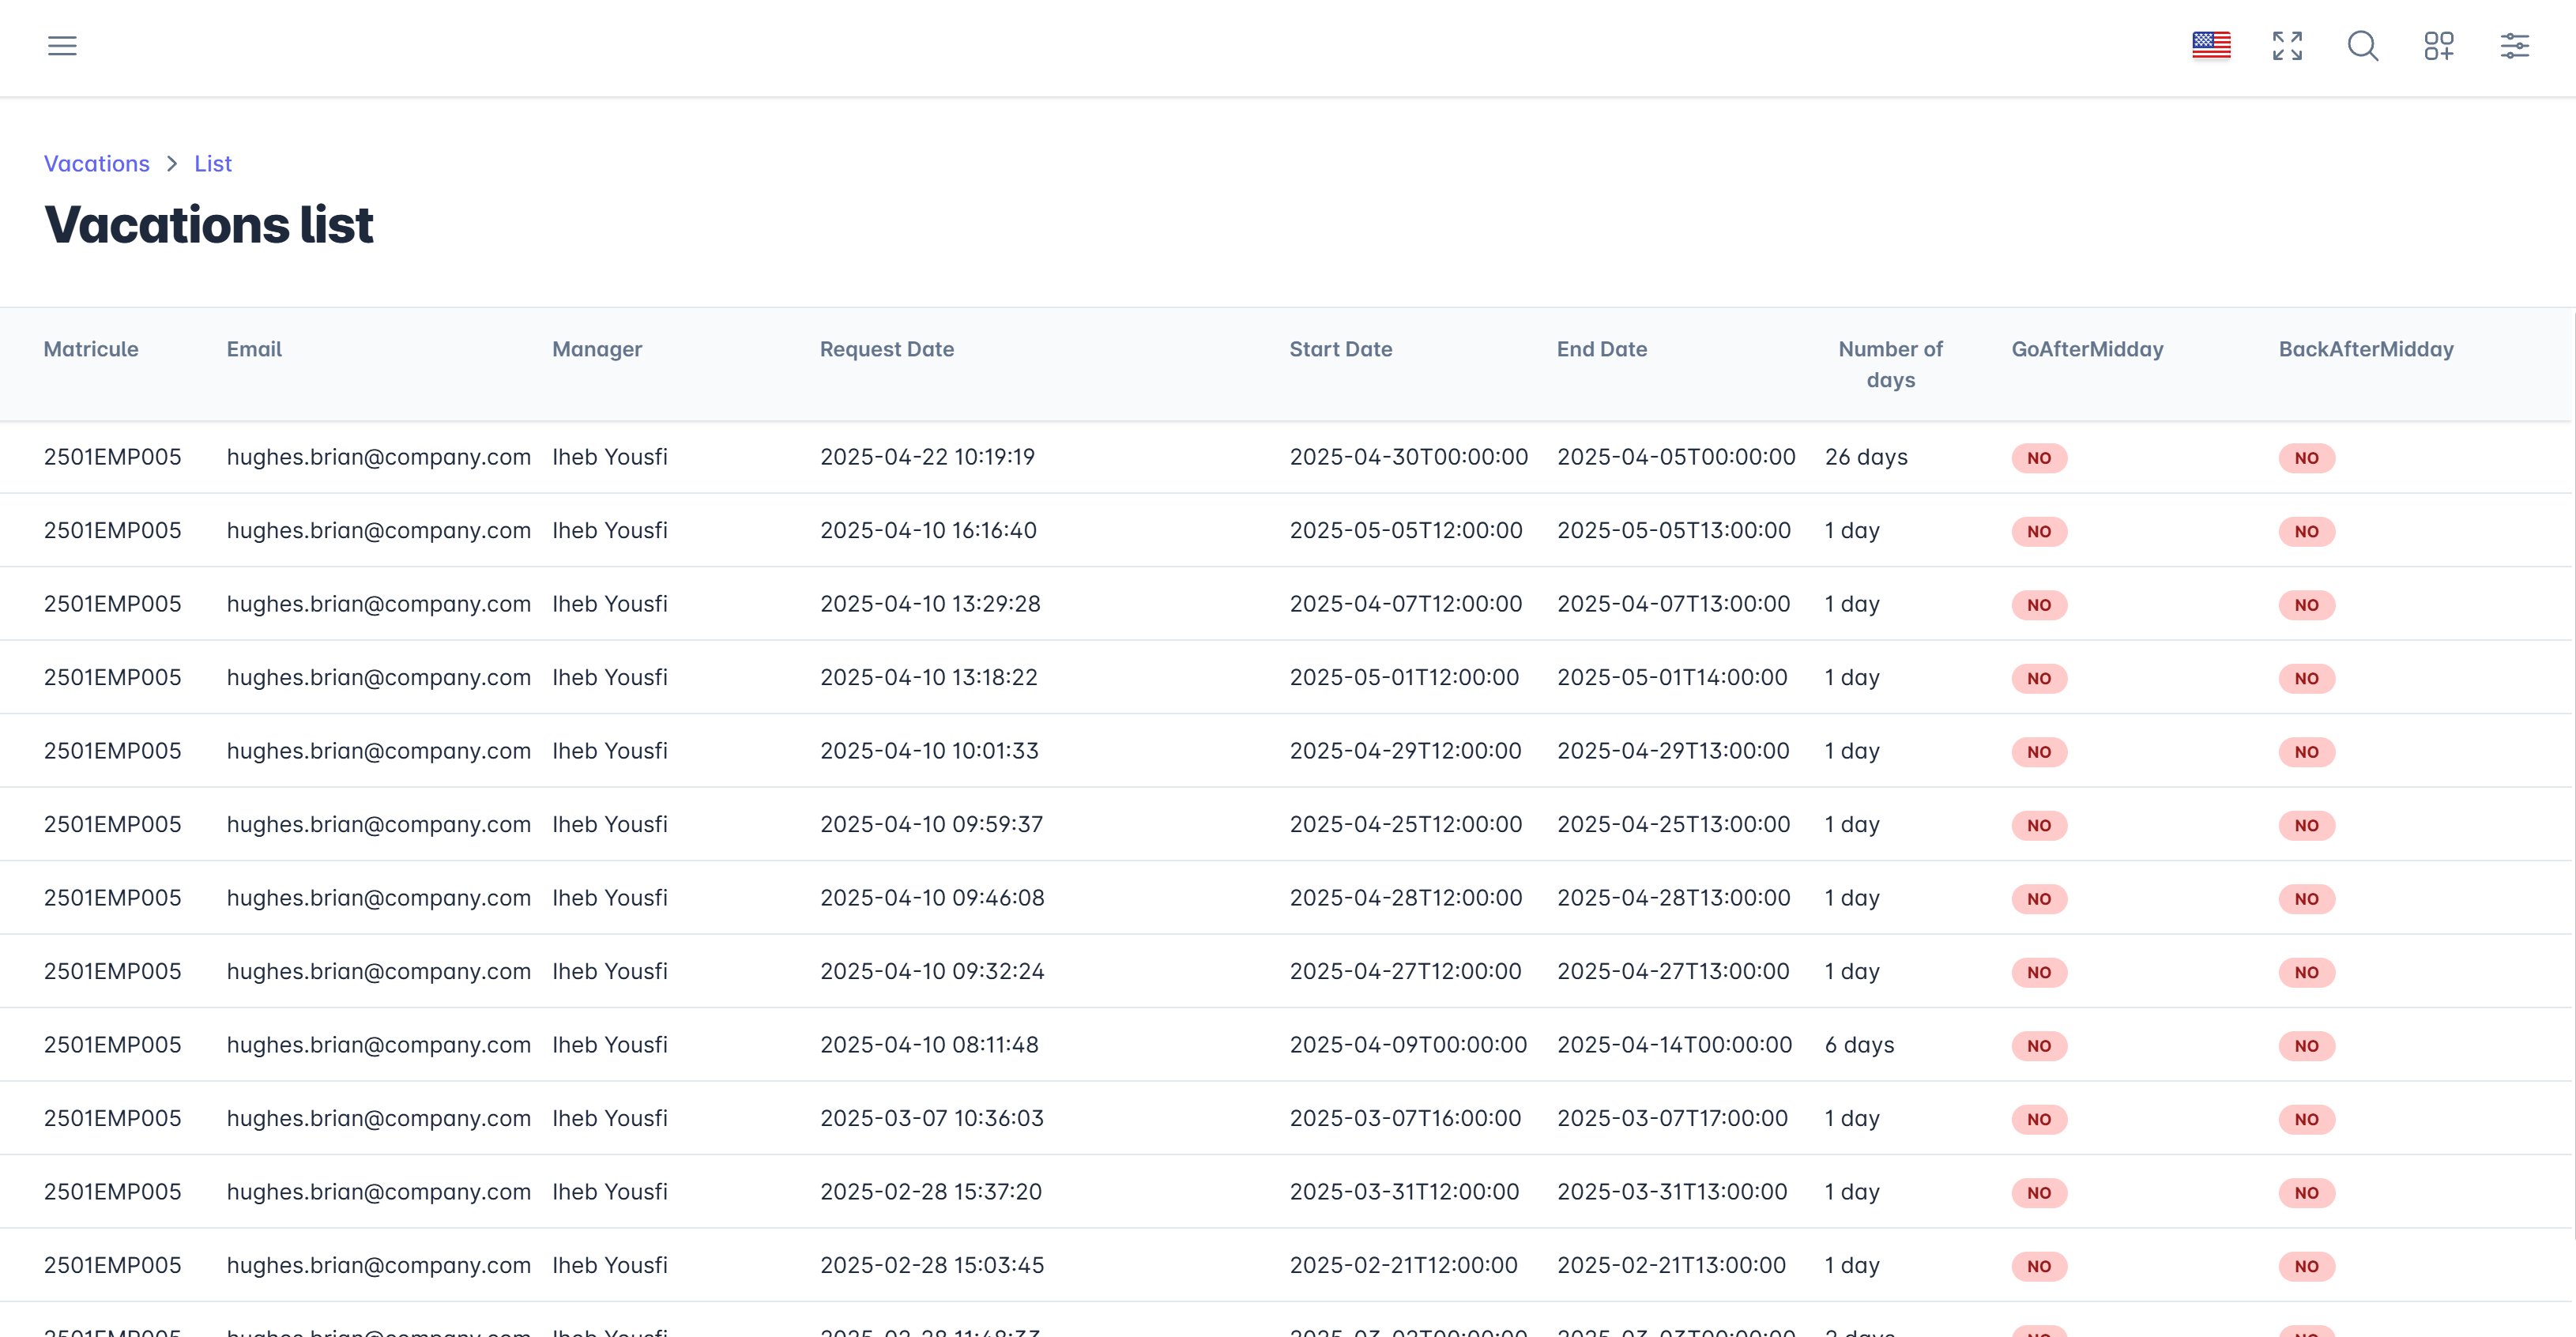
\includegraphics[width=16cm]{images/realisation/mesConges.png}
         \caption{Page de consultation des congés acceptés}
         \label{fig:ccon}
\end{figure}
\subsection{Traiter une demande}
L'interface pour traiter une demande est conçue pour permettre l'approbation ou le refus d'une demande. Le manager ou l'RH peut choisir entre deux options : accepter ou refuser la demande. Une fois la décision prise, il peut cliquer sur un bouton de validation, ce qui envoie une notification à l'utilisateur qui a soumis la demande. Les notifications peuvent être envoyées par e-mail ou par un message de notification sur la plateforme.
\newpage
\begin{figure}[h]
     \centering
     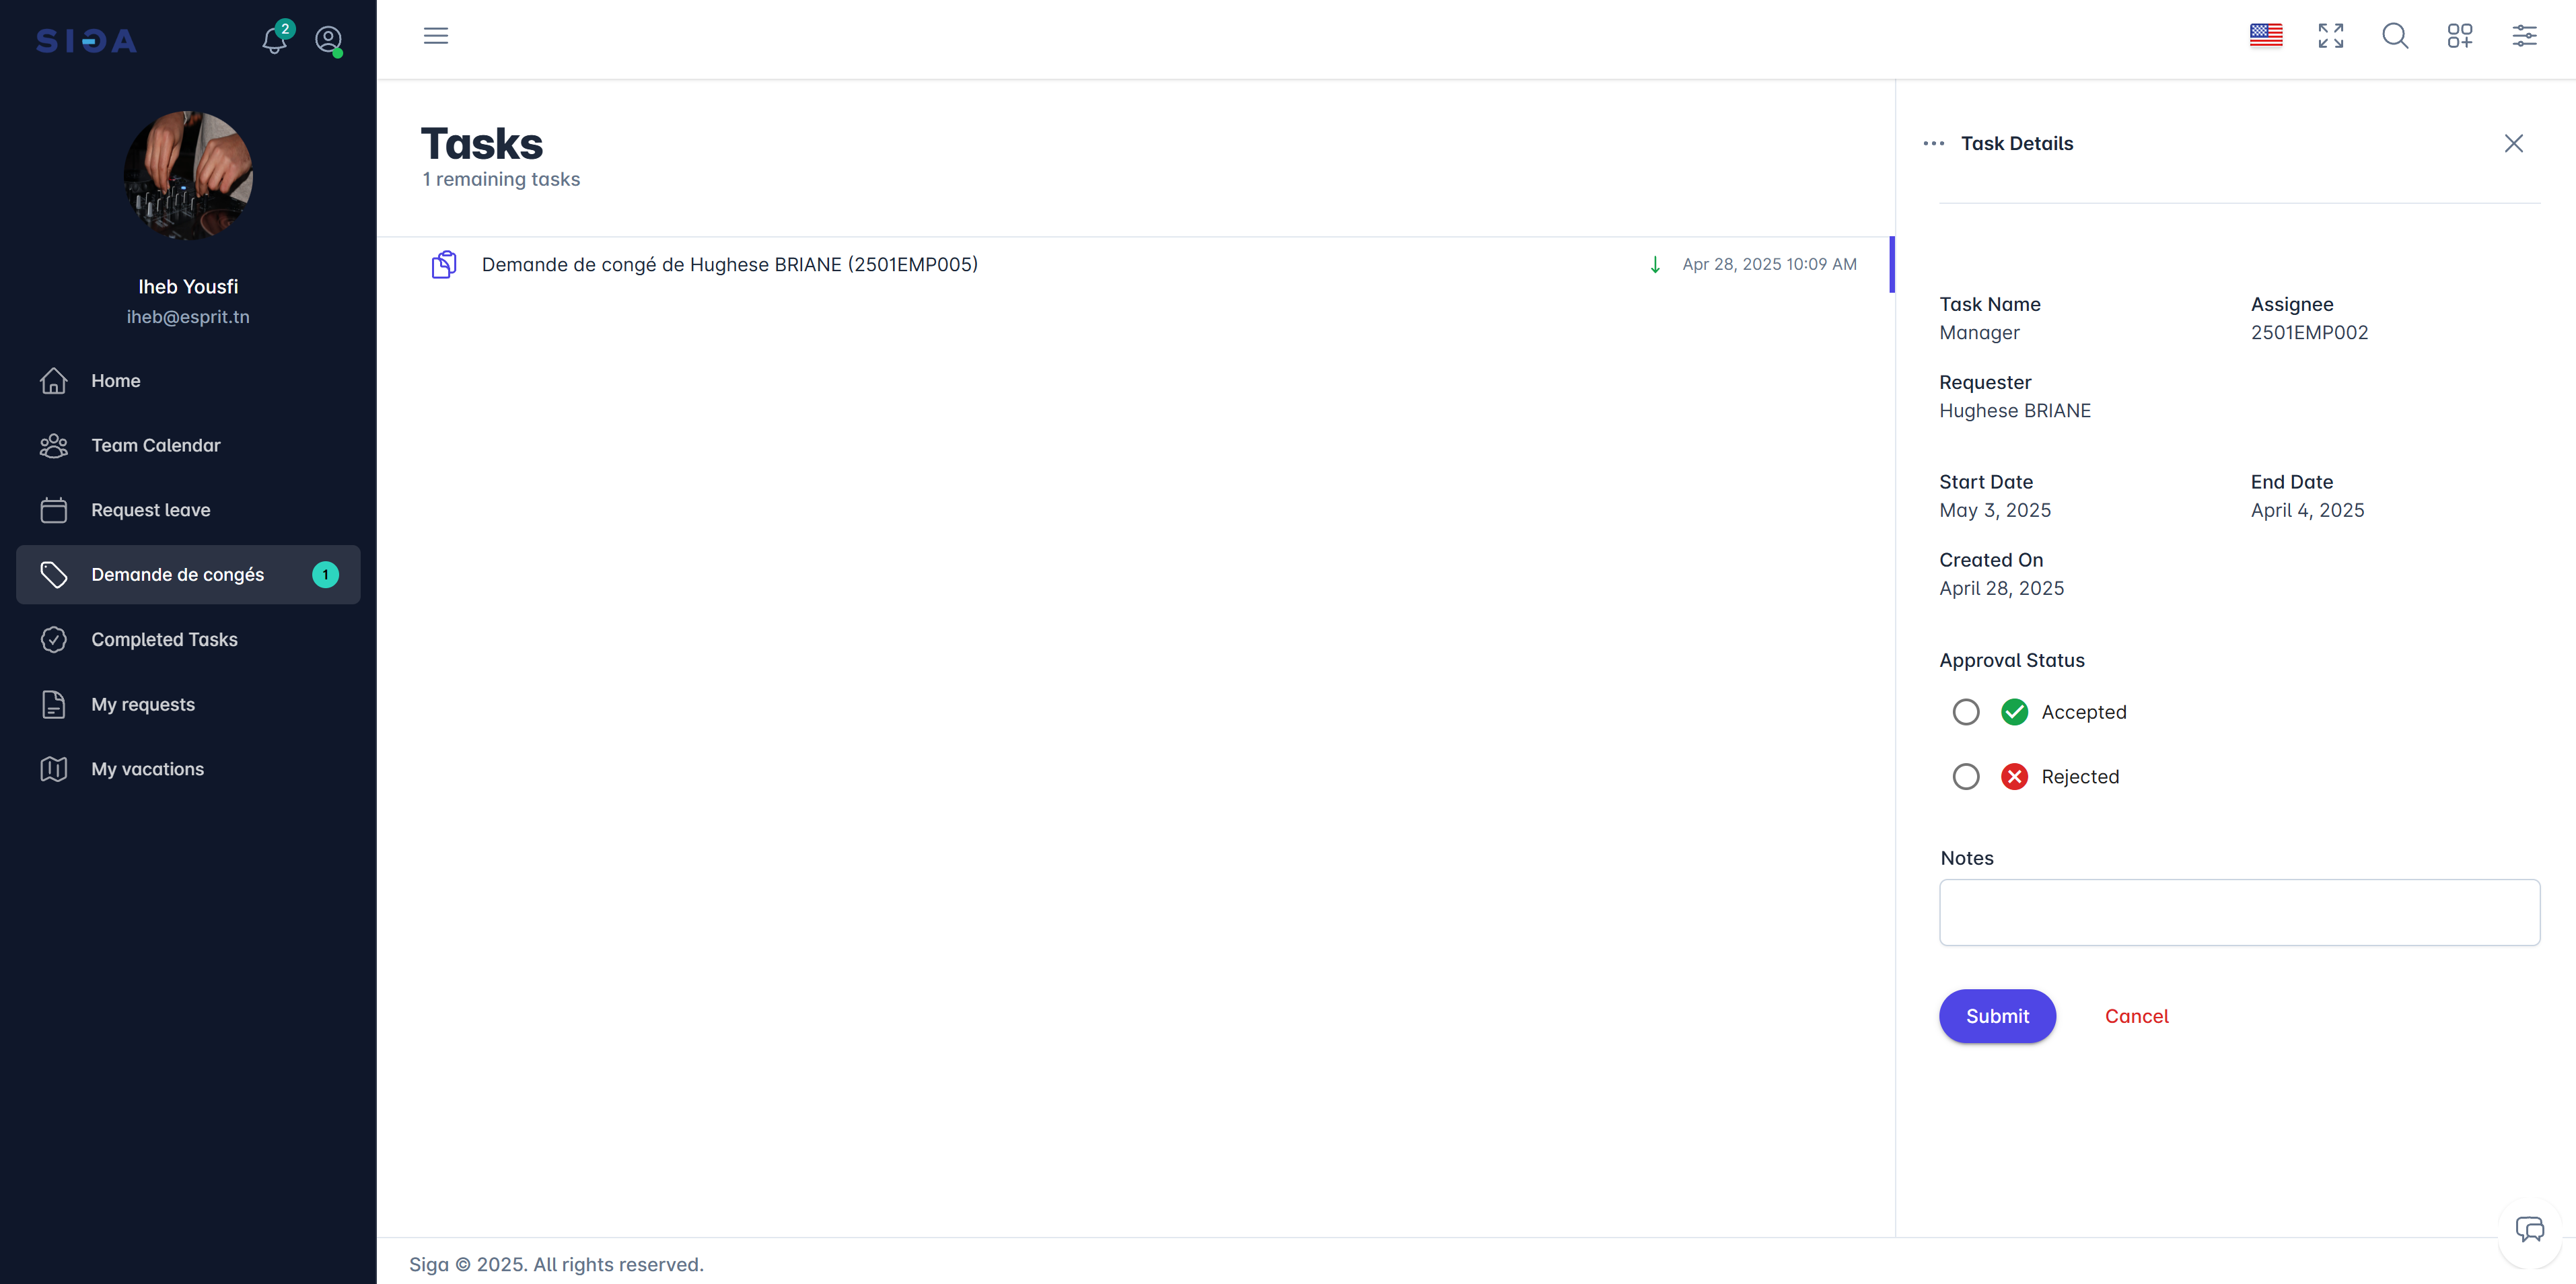
\includegraphics[width=16cm]{images/realisation/TraiterDemande.png}
     \caption{Page de traitement des demandes}
     \label{fig:traid}
\end{figure}
\section{Conclusion}
Le Sprint 2 a permis de développer des fonctionnalités essentielles pour la gestion des demandes et congés, répondant aux besoins des utilisateurs, managers et RH.

Le backlog a défini les cas d’utilisation prioritaires, raffinés via des diagrammes UML (cas d’utilisation, classes, séquences) et BPMN pour modéliser les interactions et workflows.

La conception, basée sur une architecture orientée objet et intégrant Camunda, a soutenu une réalisation réussie, avec des interfaces intuitives pour gérer les profils, réinitialiser les mots de passe, soumettre, consulter et traiter les demandes.

Ce sprint a établi une gestion efficace des demandes, ouvrant la voie à de futures améliorations comme des notifications avancées ou des tableaux de bord analytiques.